\documentclass[11pt,ngerman,parskip=half]{scrartcl}

\usepackage[utf8]{inputenc}
\usepackage[T1]{fontenc}
\usepackage{libertine}
\usepackage{babel}
\usepackage{graphicx}
\usepackage[style=authoryear-icomp,dashed=false,loccittracker=context]{biblatex}
\usepackage[thresholdtype=lines,threshold=2]{csquotes}
\usepackage{xpatch}
\usepackage{hyperref}
\usepackage{float}
\usepackage{url}
\usepackage{paralist}
\usepackage[toc,page]{appendix}
\usepackage{caption}

\makeatletter
\renewcommand\paragraph{\@startsection{paragraph}{4}{\z@}%
            {-2.5ex\@plus -1ex \@minus -.25ex}%
            {1.25ex \@plus .25ex}%
            {\normalfont\normalsize\bfseries}}
\makeatother
\setcounter{secnumdepth}{4} % how many sectioning levels to assign numbers to
\setcounter{tocdepth}{4}    % how many sectioning levels to show in ToC


\renewcommand{\appendixtocname}{Anlagenverzeichnis}
\renewcommand{\appendixpagename}{Anlagenverzeichnis}
\setlength\bibitemsep{1.5\itemsep}
\urlstyle{same}
\addbibresource{src/library.bib}
\author{}
\titlehead{
  \begin{center}
     
\includegraphics[width=0.7\textwidth]{src/img/htw-logo.pdf}
  \end{center}
}
\title{Gehirn-Computer-Schnittstellen in Neuroprothesen}

\begin{document}
\pagenumbering{Roman}
\clearpage\maketitle
\thispagestyle{empty}
\begin{tabular}{ll}
  Fachbereich: & 4 (Informatik, Kommunikation und Wirtschaft) \\
  Studiengang: & Angewandte Informatik (SoSe2018)             \\
  Seminar:     & B15 Gesellschaftliche Aspekte der Informatik \\
  Dozentin:    & Prof.-Dr. Christin Schmidt                   \\
\end{tabular}

\begin{tabular}{ll}
  Gruppe: & 5 \\
\end{tabular}

\begin{tabular}{lll}
  Gruppenmitglied        & Matrikelnummer & Kapitel\\
  Louis Knorn            & 566546         & 1\\
  John-Kevin Gold        & 566538         & 2\\
  Jeremy Etienne Seipelt & 566847         & 3\\
  Kathrin Klocke         & 514403         & 4\\
\end{tabular}

\pagebreak
\renewcommand{\baselinestretch}{0.75}\normalsize
\tableofcontents
\renewcommand{\baselinestretch}{1.0}\normalsize
\pagebreak
\listoffigures
\pagebreak

\pagenumbering{arabic}
\setcounter{page}{1}
\section{Einleitung}
Sind wir auf dem Weg zum Cyborg und werden in Zukunft mit unseren Gedanken
Exoskelette, Autos und Haushaltsgeräte steuern oder Videospiele ohne
Kontroller \enquote{zocken}? Die Se­mes­ter­ar­beit, erarbeitet in einer Gruppe,
befasst sich mit der technischen Voraussetzung dafür:
Gehirn-Computer-Schnittstelle oder engl. als Brain-Computer-Interface,
abgekürzt BCI, bezeichnet. Diese wird an der Großhirnrinde angebracht und
nimmt mittels Elektroden die Gehirnwellen auf.

Ziel der Arbeit ist es, die
Funktionsweise von BCIs sowie damit verbundenen Roboterarmen zu erläutern,
zukünftige Anwendungen zu schildern und auf ethische Aspekte der Verwendung
einzugehen. Im ersten Teil wird erklärt, wie der technische Aufbau einer BCI
und die konkrete Funktionsweise der Schnittstelle ist, sowie die
Implantierung am Menschen durchgeführt wird. Dazu wurde das Onlinearchiv PMC
genutzt um einen Überblick auf Neuroimplantate zu geben.

Darauf folgend soll
die Gerätetechnik von Gelenkarmrobotern beschrieben werden. Guittet u. a.
beschreiben in ihrer Fallstudie \enquote{The Spartacus telethesis: manipulator
control studies} aus dem Jahre 1979, dass diese Art von Roboter u.a. als
Teleoperator für Querschnittsgelähmte genutzt werden kann und auch heute
finden sich viele Artikel bei denen z.B. BCI mit Gelenkarmrobotern kombiniert
werden. Da sich neuronale Verfahren zur Bewegungssteuerung und -regelung in
diesem Bereich tendenziell noch in der Forschung befinden und Quellen nur
schwer zugänglich sind, werden die Themen Steuerung und Programmierung im
Rahmen der Belegarbeit nicht weiter behandelt.

Anschließend wird auf andere
Anwendungsgebiete der BCIs eingegangen, darunter die Verwendung für Bereiche
außerhalb der Medizin und für die Menschen im Allgemeinen und in welchen
Bereichen bereits aktiv geforscht wird. Im letzten Kapitel werden die
ethischen Aspekte und die Akzeptanz der Verwendung von BCIs untersucht. Dazu
wird zunächst auf das Thema Human Enhancement als Oberbegriff zur
Selbstoptimierung, für therapeutische und nicht therapeutisch Zwecke,
eingegangen bezugnehmend auf einen Artikel von O. Bendel in \enquote{TATuP –
Zeitschrift für Technikfolgenab- schätzung in Theorie und Praxis}. Zur
Betrachtung der ethischen Aspekte von Gehirn- Computer-Schnittstellen wird
ein Beitrag von J. Clausen für die Zeitschrift \enquote{IRIE - International Review
of Information Ethics} herangezogen. Um herauszufinden, wie aktuell die
Einstellung zu Human Enhancement und zur Nutzung einer
Gehirn-Computer-Schnittstelle ist, wurde eine Umfrage erstellt und
durchgeführt. Abschließend werden die Ergebnisse der Umfrage vorgestellt und
analysiert.

\pagebreak
\section{Die Funktion der Sensorik eines Brain-Computer-Interfaces}
Das Thema dieser Arbeit ist der Aufbau und die Funktion der Sensorik, welche
in Brain-Computer-Interfaces, zur Nutzung von Neuroprothesen, angewandt wird.
Dazu wird die invasive von den non-invasiven Methoden unterschieden,
einerseits in der Präzision, als auch in der praktischen Handhabung. Ziel
dieser Arbeit ist es, verschiedene Möglichkeiten der Erfassung von
Gehirnaktivitäten zu beschreiben. Dabei werden die Vor- und Nachteile von
non-invasiven Methoden aufgezeigt und erläutert warum die invasive Methode,
trotz hoher Gesundheitsrisiken wie Infektionen oder Hirnschäden, eine höhere
Nutzungsfrequenz im Bezug auf Neuroprothesen hat. Es wird wie folgt
vorgegangen. Zunächst wird der grobe Aufbau der Neuroprothesensteuerung
erklärt. Daraufhin wird die Funktion der Arten der Sensorik beleuchtet um ein
grundlegendes Verständnis für den Vorgang der Aufzeichnung der Hirnaktivität
zu erhalten. Abschließend werden Vor- und Nachteile verglichen.

\subsection{Aufbau des Brain-Computer-Interface} 
Das Brain-Computer-Interface (deutsch, Gehirn-Computer-Schnittstelle) ist
eine spezielle Mensch-Maschine-Schnittstelle die es ermöglicht mittels des
Nervensystems im Gehirn, eine Neuroprothese zu steuern. Das geschieht
wiefolgt: Zunächst muss der Mensch sich vorstellen die Prothese zu bewegen,
um eine Reaktion im Gehirn auszulösen. Diese Reaktion wird nun von einem
Sensor, invasiv oder non-invasiv, aufgezeichnet. Diese Signale werden nun per
Kabel an die Schnittstelle (über einen Analog-Digital-Konverter) geleitet und
analysiert. Mit genügend Übung sind Mensch und Schnittstelle dazu in der
Lage, klare Signale zu geben und auszuführen. Sollte die Schnittstelle das
Signal verstehen, wird der Befehl zu der Neuroprothese geleitet und
ausgeführt.
\parencites{uebersicht}{bciuinvasiv}

\subsection{Was sind non-invasive Sensoren}
Unter non-invasive Methoden versteht man ein Messverfahren, dass
Gehirnaktivitäten von Außen mittels Elektroden an einen Verstärker leitet um
Spannungsschwankungen sichtbar zu machen. Im Falle des
Brain-Computer-Interfaces (BCI) werden acht non-invasive Methoden genutzt.
Nur die drei häufigst genutzten werden hier erklärt.
\parencite{methoden}

\subsubsection{Elektroenzephalogramm (EEG)}
Das Elektroenzephalogramm (EEG) ist die häufigst genutzte Methode. Es misst
die elektrischen Signale ausgehend aus den Nervenzellen des Gehirns. Die
Signale werden allerdings nur mit 5-100 Mikrovolt gemessen, was dazu führt
dass ein Verstärker vonnöten ist. Um Störungen der Spannungen zu vermeiden
wird ein Differenzverstärker mit einer Gleichtaktunterdrückung genutzt. Die
gemessenen Signale werden nun digitalisiert und für eine spätere Auswertung
gespeichert.
\parencite{eegw}

\subsubsection{Funktionelle Magnetresonanztomographie (fMRT)}
Das zweite Messverfahren ist die funktionelle Magnetresonanztomographie
(fMRT). Die funktionelle Magnetresonanztomographie wird meist genutzt um
aktive Hirnareale bildlich darzustellen. Anders als bei einem EEG zum
Beispiel, werden hier nicht die elektronischen Signale gemessen. Das fMRT
misst erhöhte Mengen an sauerstoffhaltigem Blut. Diese Veränderungen des
Sauerstoffgehalts entstehen durch den erhöhten Stoffwechsel, der bei der
Nutzung der Kortexareale herbeigeführt wird.
\parencite{fmrt}

\subsubsection{Magnetenzephalographie (MEG)}
Bei der Magnetenzphalographie werden die, ähnlich wie bei dem EEG, die
magnetischen Aktivitätn via \enquote{SQUIDs} gemessen. SQUIDs
(superconducting quantum interference device) sind Sensoren die für die
präzise Messung von sehr schwachen Magnetfeldern genutzt werden. Ein SQUID
besteht aus einem supraleitendem Ring der mit normalleitendem Material
unterbrochen wird. Die Unterbrechung muss aber so dünn sein, dass die
supraleitenden Elektronenpaare noch hindurch kommen. Dieser Kontakt wird als
Josephson-Kontakt bezeichnet.
\parencite{meg}

\subsection{Was sind invasive Sensoren}
Als invasive Methode bezeichnet man das Eindringen eines Sensors in den
Neokortex. Der Grund dafür ist, dass der Neokortex der motorische Teil des
menschlichen Gehirns ist. Somit ist der Sensor in der Lage jeden
Bewegungsbefehl direkt aus dem Hirn zu entnehmen.
\parencites{bciuinvasiv}{methoden}

\subsubsection{Vorgang der Implantierung}
Das Einpflanzen des Sensors verläuft in 4 Schritten. Zunächst muss die
Schädelplatte nahe dem Neokortex geöffnet werden. Nun wird der Chip, der mit
mehreren Hundert Sensoren ausgestattet ist, mit einer Art Luftdruckpistole
wenige Millimeter in die Großhirnrinde geschossen. Dabei muss besondere
Vorsicht geboten werden, da bei Fehlern die Chance auf eine Hirnblutung sehr
hoch ist. Nun muss der Sensor mit der Schnittstelle verbunden werden (per
Kabel oder Funk). Zu guter Letzt wird die Schädelplatte wieder an den Kopf
angebracht. Ein weiteres Problem ist, es kann vorkommen dass die Sensoren
nachjustiert werden müssen. Das führt dazu dass die Schädeldecke weitere male
geöffnet werden muss, was wiederum die Chance auf eine Infektion im Gehirn
erhöht.\cite{bciuinvasiv}

\subsection{Vor und Nachteile}  
\subsubsection{fMRT}
Da die funktionelle Magnetresonanztomographie den Sauerstoffgehalt in aktiven
Gehirnarealen misst, ist die fMRT auf den erhöhten Blutfluss angewiesen.
Dadurch entsteht folgendes Problem. Die Messung der Reaktion im Gehirn ist
zwar präzise was den Ort angeht, hat jedoch eine zeitliche Verzögerung und
Ungenauheiten bei kurzen Bewegungen. Das bedeutet, man kann einfache Befehle
wie \enquote{Arm hoch} oder \enquote{Arm runter} geben. Man verliert durch
die Verzögerung allerdings das Gefühl für das kontrollieren der Prothese.

\subsubsection{MEG}
Die Magnetenzophalographie misst, wie das Elektroenzophalogramm, die
elektromagnetischen, von den Hirnzellen ausgehenden, Signale. Das hat den
Vorteil, dass es nicht wie bei der funktionellen Magnetresonanztomographie zu
Verzögerungen kommt. Durch den Einsatz der \enquote{SQUIDs} kann die
Schnittstelle außerdem mit relativ präzisen Befehlen versorgt werden. Der
größte Nachteil ist jedoch, dass die Geräte nicht nur statisch sind, sonder
auch sehr teuer. Zusätzlich benötigt man für den Dauerbetrieb ca. 400l
flüssiges Helium pro Monat zur Kühlung. Das heißt, diese Geräte können für
die Forschung der Neuroprothesen genutzt werden, haben jedoch keine Zukunft
für die praktische Anwendung.

\subsubsection{EEG}
Das Elektroenzophalogramm ist das meist genutzte non-invasive Messverfahren
im Bezug auf Neuroprothesen. Die Gründe dafür sind, dass ein
Elektroenzophalogramm vergleichsweise günstig ist. Eine Art Badekappe, einige
Sensoren und Kabel sind alles was benötigt wird um eine relativ präzise
Messung vorzunehmen. Dies reicht häufig aus, um simple Neuroprothesen
einigermaßen gut zu steuern.So verbreitet das Elektroenzophalogramm auch ist,
allein dadurch, dass es außerhalb des Gehirns angebracht wird, fehlt es dem
EEG an Präzision um genug Informationen für feinmotorische Aktionen zu
liefern. Für diese Aktionen wird ein, im Gehirn angebrachter Sensor benötigt.
Nur so (beim derzeitigen technischem Stand) ist man dazu in der Lage mit
intensivem Training eine Neuroprothese verlässlich zu kontrollieren. Die
einzigen Nachteile dabei sind erstens, das Problem, dass der Sensor weiterhin
eine Kabelverbindung benötigt. Die Forschung für eine Funkverbindung ist
allerdings bereits im Gange. Zweitens, die medizinischen Risiken, die sich
auf Hirnblutung während der Implantierung und Infektionen durch wiederholtes
Öffnen der Schädeldecke beziehen.

\subsection{Fazit}
Zum Schluss lässt sich nurnoch sagen, dass die Sensorik noch zu wünschen
lässt. Sowohl in der Genauigkeit der Daten, als auch in Handhabung und
gesundheitlichen Risiken. Dies sollte aber nicht allzu problematisch sein.
Die Menschheit hat technologisch in den letzten Jahren sehr viel erreicht.
Vor 50 Jahren hätte Niemand auch nur erahnen können, dass eine Prothese mit
den eigenen Gedanken gesteuert werden kann. Wer weiß schon was in den
nächsten 50 jahren technologischem Fortschritt passiert? Aber wir scheinen
auf dem besten Weg zu sein, Taube wieder hören zu lassen und Gelähmten die
Möglichkeit zu geben wieder zu laufen.
\parencites{eegw}{fmrt}{meg}{bciuinvasiv}

\pagebreak
\section{Funktionsweise der Gerätetechnik von Gelenkarmrobotern}
\label{sec:john}
\subsection{Einführung}
\label{subsec:john_einfuehrung}
Der Artikel \enquote{Neuroprothese: Gelähmter steuert Roboterarm mit bloßer
Vorstellungskraft} aus dem Jahr 2015 beschreibt, wie ein Mensch einen
Industrieroboter-ähnlichen Gelenk- bzw. Knickarmroboter mittels eines
Brain-Computer-Interface steuert
\parencite[vgl.][]{merkelt_neuroprothesen:_2015}. Die Idee, verlorene oder
gelähmte Gliedmaßen durch Roboterarme zu ersetzen, ist allerdings nicht völlig
neu. Bereits im Jahr 1979 veröffentlichten Guittet u. a. eine Fallstudie, die
eine vergleichbare Anwendung untersuchte. Man bezeichnete einen solchen
Roboterarm auch als Telethese, allerdings wurde der Arm damals durch einfache
Kopfbewegungen kontrolliert \parencite[vgl.][]{guittet_spartacus_1979}.

\begin{figure}[H]
  \centering
  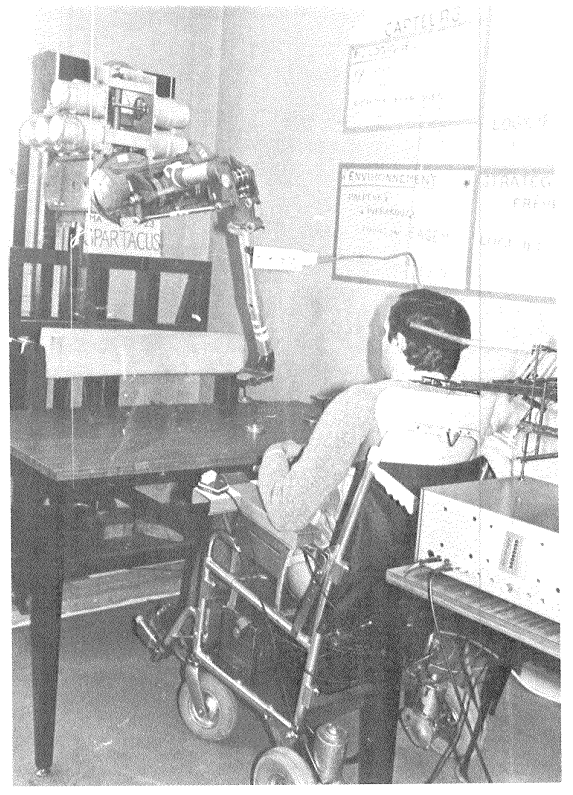
\includegraphics[width=0.6\textwidth]{src/img/john1.png}
  \caption{Knickarmrobotersteuerung durch Kopfbewegungen}
  \label{img:john1}
  \parencite[][84]{guittet_spartacus_1979}
\end{figure}
\pagebreak

Nachdem im ersten Kapitel der Gruppenarbeit die Funktionsweise von BCI
erläutert wurde, beschäftigt sich der folgende Abschnitt mit der
Gerätetechnik eines Gelenkarmoboters sowie Begriffen und Grundlagen der
Robotik im Allgemeinen. Die Gerätetechnik gehört zu den Kernkomponenten in
einem Robotersystem und beinhaltet technische Elemente für Kinematik,
Sensorik und Aktorik. Zu den weiteren Kernkomponenten, die im Rahmen der
Belegarbeit nicht weiter behandelt werden, zählen:
\begin{compactitem}
  \item Steuerung (z.B. Rechnerkopplung, Interpolation)
  \item Programmierung (z.B. Punkt- und Bahnsteuerung, Prozessbeschreibung)
  \item Prozessführung (Geometrie- und Technologiedatenverarbeitung, Steuer-
        und Regelstrategie)
  \item Endeffektor (z.B. Greifer, Werkzeuge)
\end{compactitem}
\parencite[vgl.][40]{hesse_taschenbuch_2016}

Der Begriff Robotik ist laut DIN definiert als:
\blockquote[{\cite[DIN EN ISO 8373, zitiert nach][39]
{hesse_taschenbuch_2016}}]{Robotertechnik, zu der man Entwurf und
Berechnung, Herstellung, Steuerung von Robotern, Einsatz in Standard- und
Problemlösungen, Erforschung von Steuerungsvorgängen bei Mensch und Maschine,
Sensoren und Endeffektoren sowie deren Anwendung zählt}.
Roboter können nach verschiedenen Kriterien, wie Anwendungsbereich,
Einsatzgebiet, Ausführung und Aufgaben, gruppiert werden
\parencite[vgl.][25\psq]{hesse_taschenbuch_2016}. Die VDI-Richtlinie 2860
beschreibt Industrieroboter beispielsweise wie folgt:
\blockquote[{\cite[VDI-Richtlinie 2860, zitiert nach][16]
{weber_industrieroboter:_2017}}]{Industrieroboter sind universell
einsetzbare Bewegungsautomaten mit mehreren Achsen, deren Bewegungen
hinsichtlich Bewegungsfolge und Wegen bzw. Winkeln frei programmierbar (d.h.
ohne mechanischen Eingriff vorzugeben bzw. änderbar) und gegebenenfalls
sensorgeführt sind. Sie sind mit Greifern, Werkzeugen oder anderen
Fertigungsmitteln ausrüstbar und können Handhabe- oder andere
Fertigungsaufgaben ausführen}.

Roboter, insbesondere Industrieroboter, können demnach auch als
Handhabungsgeräte bzw. -technik betrachtet werden.
Abbildung~\ref{img:john2} zeigt, dass
Handhabungsgeräte primär in manuell gesteuerte oder programmgesteuerte Geräte
eingeteilt werden können. Es gibt darüber hinaus aber auch Mischformen in der
Robotik, z.B. beim Serviceroboter. Dieser ist ein Hybrid aus Industrieroboter
und Manipulator, welcher Dienstleistungen für den Menschen erbringt.
Serviceroboter reagieren auf menschliche Anweisungen (manuelle Steuerung)
führen Teilaufgaben aber auch automatisch bzw. programmgesteuert aus.
\parencite[vgl.][15--17]{weber_industrieroboter:_2017}

\begin{figure}[H]
  \centering
  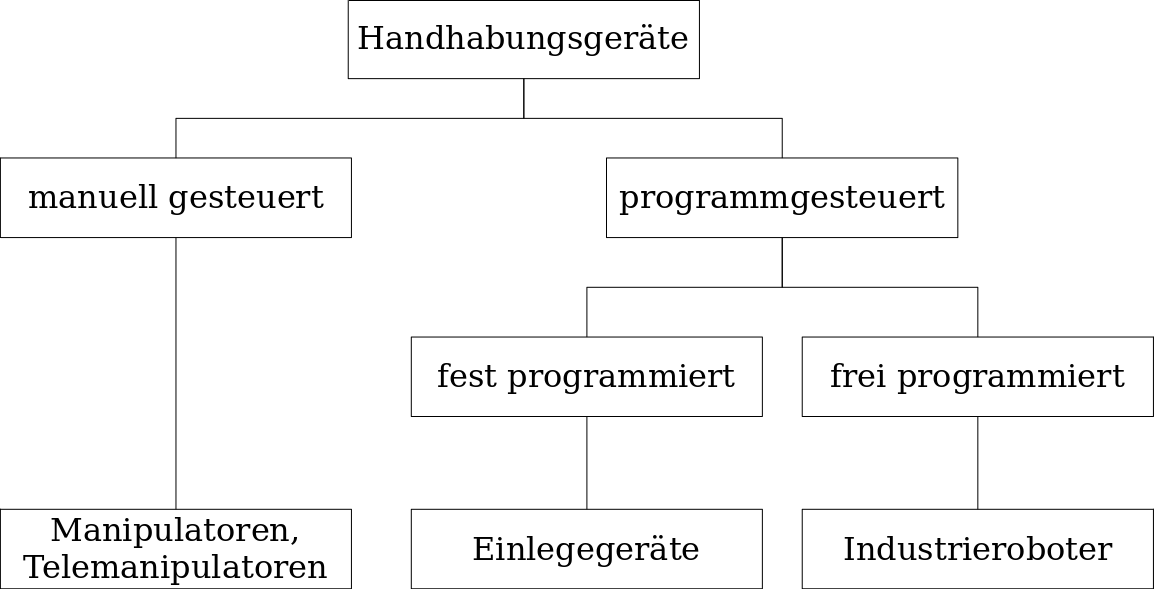
\includegraphics[width=0.7\textwidth]{src/img/john2.png}
  \caption{Einteilung von Handhabungsgeräten}
  \label{img:john2}
  \parencite[][16]{weber_industrieroboter:_2017}
\end{figure}

\subsection{Kinematik}
\label{subsec:john_kinematik}
Die Anordnung der Armteile und Gelenke bestimmt die kinematische Struktur
eines Roboters, hierbei unterscheidet man hauptsächlich zwischen serieller
Kinematik und Parallelkinematik. Roboter die aus einer Aneinanderreihung von
Armteilen bestehen, welche wiederum durch Gelenke bzw. Achsen verbunden sind,
ordnet man der seriellen Kinematik zu. Das letzte Armteil in einer solchen
Anordnung, kann auch als Effektor bzw. Endeffektor bezeichnet werden. Hierbei
handelt es sich um das Teil des Roboters, welches in Kontakt mit der Umgebung
tritt, um z.B. Objekte zu greifen. Bei der Parallelkinematik hingegen sind
mehrere Schub- oder Drehgelenke mit dem Effektor verbunden und wirken direkt
auf diesen. Der Gelenkarmroboter weist eine serielle Kinematik auf. Die
kinematische Struktur eines Roboters bestimmt wiederum seinen Freiheits- bzw.
Getriebefreiheitsgrad. \parencite[vgl.][17--20]{weber_industrieroboter:_2017}

Der Freiheitsgrad \textit{f} beschreibt
\textquote[{\cite[][18]{weber_industrieroboter:_2017}}]{[...] die Anzahl der
möglichen unabhängigen Bewegungen (Verschiebungen, Drehungen) eines starren
Körpers gegenüber einem Bezugssystem}. Es gibt hierbei zwei wesentliche
Grundbewegungen, die Translation (Gleit- oder Verschiebebewegung) und die
Rotation (Drehbewegung). Bei der Translation bewegt sich der Körper
theoretisch ohne sich selbst zu drehen (starr) entlang einer oder mehrerer
Raumachsen (x-, y- und z-Achse). Bei der Rotation hingegen dreht sich der
Körper um einen bestimmten Mittelpunkt bzw. um eine bestimmte Achse, die
innerhalb oder außerhalb des Körpers liegen kann.
\parencite[vgl.][53\psq]{schunke_funktionelle_2014}

Abbildung~\ref{img:john3} stellt die Freiheitsgrade am
Beispiel der Bewegungsmöglichkeiten eines Tennisballs im Raum dar.
\begin{figure}[H]
  \centering
  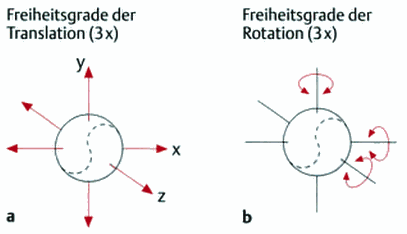
\includegraphics[width=0.6\textwidth]{src/img/john3.png}
  \caption{Translation (a) und Rotation (b)}
  \label{img:john3}
  \parencite[][53]{schunke_funktionelle_2014}
\end{figure}

Der Getriebefreiheitsgrad F gibt an,
\textquote[{\cite[][18]{weber_industrieroboter:_2017}}]{[...] wie viele
unabhängig voneinander angetriebene Achsen zu einer eindeutigen Bewegung des
Roboterarms führen}. Bei Gelenkarmrobotern mit sechs Achsen (F=6), kann der
Effektor durch geschickte Anordnung der Gelenke, den maximalen Freiheitsgrad
f=6 erreichen. Roboter können generell aber auch mit mehr als sechs Achsen
(F>6) konstruiert werden, dies bezeichnet man als redundante Kinematiken.
Hierdurch erzielt man auf Kosten eines erhöhten Steuerungsaufwands eine
Verbesserung der Feinbewegungen.
\parencite[vgl.][18]{weber_industrieroboter:_2017}

Abbildung~\ref{img:john4} zeigt die Drehrichtung der Roboterachsen des
Gelenkroboters KUKA KR AGILUS sixx.
\begin{figure}[H]
  \centering
  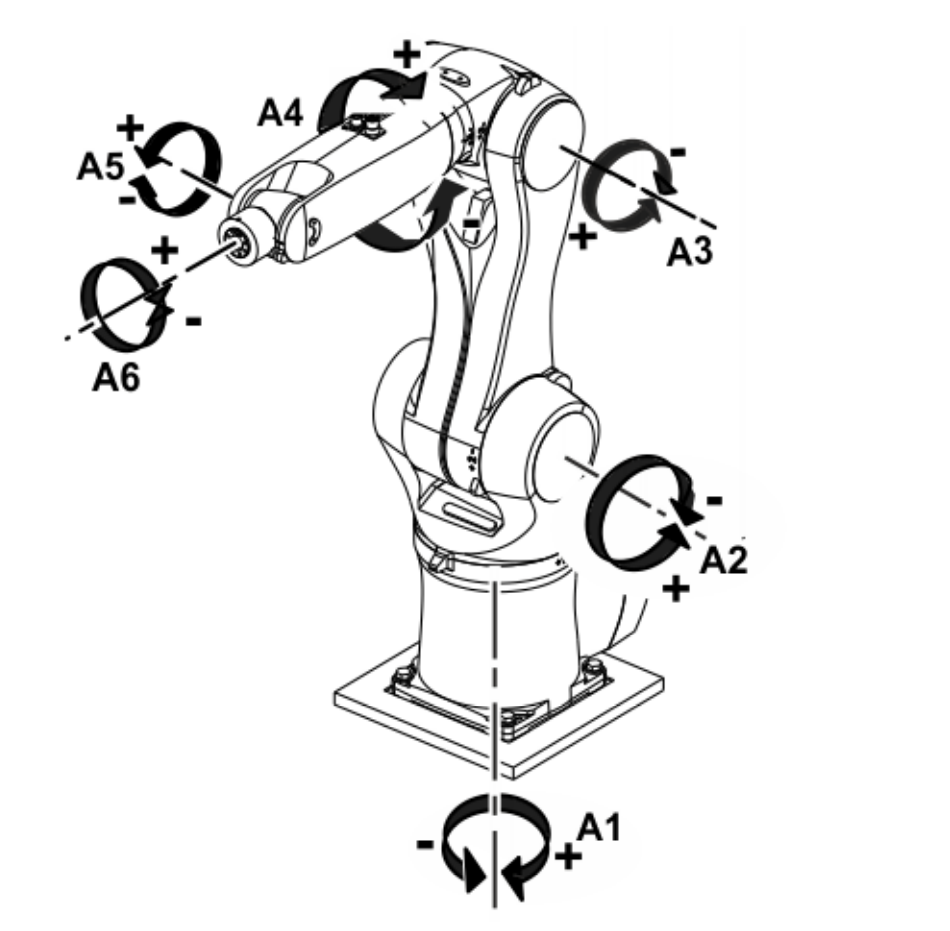
\includegraphics[width=0.5\textwidth]{src/img/john4.png}
  \caption{KR AGILUS sixx}
  \label{img:john4}
  \parencite{kuka_gmbh_kr_2018}
\end{figure}

\subsection{Aktorik}
\label{subsec:john_aktorik}
Gelenkmodule und Achsverbindungen werden durch die Aktorik eines Roboters
angetrieben und ermöglichen somit die Bewegung des Effektors. Der Aktor hat
demnach die Aufgabe eine Achse von einer Position auf eine andere zu bewegen,
hierzu gibt es vier typische Betriebszustände:
\begin{compactitem}
  \item Antrieb und Beschleunigung im Rechtslauf
  \item Abbremsung im Rechtslauf
  \item Antrieb und Beschleunigung im Linkslauf
  \item Abbremsung im Linkslauf
\end{compactitem}

Zu den wesentlichen Gruppen in der Aktorik gehören pneumatische oder
hydraulische Aktoren (z.B. doppeltwirkende Zylinder oder Druckluftmotoren)
sowie elektrische Aktoren (z.B. bürstenbehaftete und bürstenlose
Gleichstrommaschinen). Jede Gruppe hat ihre individuellen Vor- und Nachteile,
weshalb in einem Robotersystem, und so z.B. auch bei einem Gelenkarmroboter,
verschiedene Kombinationen von Aktoren zum Einsatz kommen können. Generell
lässt sich festhalten, dass pneumatische und hydraulische Aktoren die
höchsten Kräfte erzielen und daher sehr hohe Geschwindigkeiten erreichen
können, allerdings erreichen sie nicht die hohe Positioniergenauigkeit von
elektrischen Aktoren.
\parencite[vgl.][63--79]{hesse_taschenbuch_2016}

Neben dem eigentlichen Antrieb bzw. Motor sind auch Getriebe teil der Aktorik
in einem Roboter. Getriebe sind notwendig, da die Bewegungen der Aktoren
nicht immer direkt den Anforderung des mechatronischen Systems entsprechen.
Sie dienen allgemein der Übertragung und Umformung von Bewegungen sowie von
Kräften, mittels der Änderung von Drehmomenten, -richtungen oder der
Umsetzung einer Drehbewegung in eine Linearbewegung. Auch hier gibt es viele
verschiedene Bauformen, deren Anwendung je nach Anforderung variiert, z.B.
Kugelumlaufspindeln, Planetengetriebe, Kegelradgetriebe oder Zahnriemengetriebe.
\parencites[vgl.][121\psq]{maccloy_robotertechnik:_1989}
[][89--96]{hesse_taschenbuch_2016}

\subsection{Sensorik}
\label{subsec:john_sensorik}
Die Sensorik in einem Robotersystem ermittelt inner- und außerhalb des
Systems vorliegende Informationen. Dies ist erforderlich um die komplexen
Bewegungsabläufe in einer nur teilweise bestimmbaren Umwelt auszuführen. Die
Robotik stützt sich dabei häufig auf Erkenntnisse aus der Bionik\footnote{
Die Bionik erforscht wie biologische Phänomene auf technische Systeme
übertragen werden können. \parencite[vgl.][]{feess_definition:_2018}} und man
unterscheidet primär zwischen internen (interozeptiven bzw. propriozeptiven)
und externen (exterozeptiven) Sensoren. Interozeptive Sensoren messen interne
Zustände wie Motorgeschwindigkeit, Ladezustand oder Greifkraft und
exterozeptive Sensoren ermitteln Informationen aus der Umgebung, z.B. zur
Entfernungsmessung von Objekten. Nutzt ein Sensor dabei nur die Energie bzw.
Signale aus der Umgebung, bezeichnet man ihn auch als passiven Sensor (z.B.
Kameras oder Kontaktsensoren). Aktive Sensoren hingegen senden Energie aus
und messen die Reaktion der Umgebung darauf (z.B. Laser- \&
Ultraschallscanner sowie Infrarotsensoren).
\parencites[vgl.][23\psq]{hertzberg_mobile_2012}[][73]
{kruse_mehrobjekt-zustandsschatzung_2013}[][97]{hesse_taschenbuch_2016}

Zu den wesentlichen Aufgaben der Sensorik zählen:
\blockquote[{\cite[][97]{hesse_taschenbuch_2016}}]{
  \begin{compactitem}
    \item Bewegungsüberwachung (z.B. Abgleich- und Justiervorgänge)
    \item Bewegungssteuerung (z.B. Konturverfolgung)
    \item Kraftsteuerung (z.B. Einpressen, Zusammenstecken)
    \item Sensorgesteuertes Erreichen einer Zielposition (unbekannte Position
          und Orientierung eines Teils)
    \item Programmablaufkontrolle (z.B. selektive Montage)
    \item Überwachung von Endeffektoren (z.B. Greifkraft, Rutschsensor)
  \end{compactitem}
}

Zu den wichtigsten Sensoren gehören Positionssensoren,
Beschleunigungssensoren und Sensoren zur Kräftemessung. Positionssensoren
ermitteln die Position bewegter Komponenten wie dem Endeffektor und lassen sich
z.B. durch inkrementale Weg- und Winkelgeber, Resolver oder elektrische Kompasse
realisieren. Zur optischen Positionsmessung gibt es neben Kameras eine Vielzahl 
von Lasersensoren mit unterschiedlichen Funktionsweisen wie
Laserlaufzeitmessung, Lasermodulation, -triangulation oder -interferometrie.
Beschleunigungssensoren messen Beschleunigungen und Rotationsraten, um die
aktuelle Position und Orientierung eines betrachteten Körpers ausgehend von
einer bestimmten Startposition zu berechnen. Hier kommen z.B. elektrische
oder optische Gyroskope zum Einsatz. Zur Kräftemessung werden in der modernen
Robotik Kraft-Moment-Sensoren eingesetzt, welche in der Regel alle drei
Raumkräfte und -momente messen. Die Messung erfolgt dabei über
piezoelektrische Elemente oder Dehnmessstreifen.
\parencite[vgl.][98--117]{hesse_taschenbuch_2016}

\subsection{Fazit}
\label{subsec:john_fazit}
Roboter sind höchst komplexe mechatronische Systeme, die primär aufgrund
ihrer industriellen Nutzung weiterentwickelt wurden. Es hat sich gezeigt,
dass der Effektor eines Gelenkarmroboters im Vergleich zu anderen
kinematischen Strukturen den höchsten Freiheitsgrad erreichen kann. Daraus
begründet sich auch der geeignete Einsatz als Telethese. Allerdings konnten
im Rahmen der Belegarbeit viele wichtige Fragen, wie beispielsweise zur
Steuerung, Prozessführung oder den Endeffektoren, nicht geklärt werden. In
Anbetracht der Komplexität von Robotersystemen stellt sich auch die Frage
nach sicherheitstechnischen Anforderungen, insbesondere wenn solche Systeme
als Prothesen genutzt werden. Während bei stationären Industrierobotern z.B.
umzäunte Sperrbereiche eingerichtet werden können, bestünde im Fall von
Fehlfunktionen bei einem mobilen Roboterarm die Gefahr Lebewesen oder Objekte
im unmittelbaren Umfeld oder den Anwender selbst zu verletzen.

\pagebreak
\section{Anwendungsmöglichkeiten für BCIs in nicht-medizinischen Bereichen}
\subsection{Einleitung}
BCIs werden mit großem Fokus auf die Medizin/Neurowissenschaften entwickelt
\footnote{Aussage wurde allein über die Anzahl an Artikel, denen ein starker
Fokus im med./neur. Bereich anhand des Titels anzusehen ist, die die BBCI
unter den Publikationen auflistet. Alle Publikationen die für diese Arbeit
verwendet wurden sind unter http://bbci.de/publications.html aufgelistet.}.
Bereits heute sind rudimentäre Prothesen mit intrusiven Methoden möglich
sowie das Auslesen/Übertragen von Gehirnwellen mit dem weniger intrusiven
Berlin BCI. Dabei werden mit verschiedenste Methoden unterschiedliche
Gehirnaktivitäten ausgelesen und für die Weiterverarbeitung am Computern
vorbereitet.\\ Der Fokus dieser Arbeit liegt auf einem Überblick der
Anwendungsmöglichkeit außerhalb der Medizin und Neurowissenschaft. Dabei geht
es in dieser Arbeit um die folgenden zwei Gebiete, Datengewinnung,
Peripherie. Diese Arbeit soll nur eine Übersicht der derzeitigen Arbeiten an
den genannten Gebieten geben, deshalb wird kein moralisches Urteil über die
vorgestellten Methoden/Einsatzmöglichkeiten ein Teil dieser Arbeit sein. Zu
jedem Bereich wird im jeweiligen Bereiche vorstellbare, jedoch nicht im
Umfang der Recherche gefundenen, Anwedungen angegeben.

\subsection{Datengewinnung}
Unter allgemeinen Datenverwendung ist im Verlauf der Arbeit alle
Anwendungsgebiete gesammelt, bei der die Daten des BCIs ausgewertet weden um
Entscheidungen zu fällen oder einen Datensatz zu erstellen.

\subsubsection{Entscheidungshilfe}
In dem Artikel ''Implicit relevance feedback from electroencephalography and
eye tracking in image search''\parencite{tracking} der sich mit der
Realisation von gedankenunterstützem Navigieren über Suchergebnisse von
Suchmachinen für Bilder beschäftigt, spricht man von der Möglichkeit mithilfe
des Gehirns die subjektive Relevanz der einzelnen Ergebnisse herauszufiltern.
Ein weiterer Teil der Arbeit ist die Untersuchung ob Eye Tracking im verbund
mit dem BCI ein besseres Ergebniss erzielt als jeweils für sich. Hierbei wird
mithilfe eines BCIs bei einer Suche nach einem Begriff, der sich in zwei
Kategorien einteilen lässt, die Ergebnisse der gesuchten Kategorie anhand der
Signale des BCIs klar von anderen Ergebnissen abgehoben. Die Präzesion des
BCIs alleine lag bei $76.9\% \pm 8.7\% $ des EyeTracker bei $81.0\% \pm 6.7\%
$ und kombiniert bei $85.9\% \pm 5.8\% $\parencite[3.1.]{tracking}. Damit
wurde gezeigt das die BCI Technologie wirksamerweise komplementär mit einem
Eyetracker eingesetzt werden kann um Entscheidungen zu treffen.

\paragraph{Neuromarketing}
Die Idee hinter Neuromarketing ist das durch zbs. BCIs von Konsumenten noch
weitere Informationen sammeln lässt. Neuromarketing lässt sich deshalb
definieren als mit Neurologischen Messmethoden auf die Produktakzeptanz des
Endverbrauchers zu schließen, jedoch ist die Wissenschaft sich noch uneinig
was man alles unter den Begriff des Neuromarketing
zusammenfasst\parencite{marketing,beyond}. Da die Verwendung von BCIs jedoch
die Kosten von Marketingmaßnahmen erhöhen und ein Beweiß der Effektivität
solcher Technologien im Marketing nicht bewiesen sind, wird davon ausgegangen
das diese nicht in näherer Zukunft angewandt werden, da noch keine genauere
Forschung über das Thema zur Verfügung stand.

\paragraph{Qualitätssicherung}
Die BCIs erlauben uns in der Qualitätssicherung Eigenschaften zu testen ohne
einen Probanden zu befragen, so wird von Arndt behauptet das die Daten des
BCIs unterschiedlich bei dem selben Bild in unterschiedlicher Qualität
ist\parencite{video}. Diese Eigenschaft ließe sich dann auf andere Arten der
Qualitätsicherung Anwenden um neue Kriterien der Qualitätssicherung zu
erstellen, und neben bereits etablierten Methoden komplementär zum Einsatz
kommen.

\subsubsection{Benutzerstatus}
Wenn man von User State spricht so spricht man von dem derzeitigen Status des
grade untersuchtem Probanden. Anhand von User States soll man in Zukunft in
vielen Bereichen den derzeitige Status mithilfe on BCIs messen können um
anhand der Werte bestimmte Entscheidungen zu treffen. Als Beispiel wird die
\enquote{Schläfrigkeit} eines Autofahrers genannt bei dem die BCI messwerte
komplementär mit einem Pulsmesser benutzt werden könnte. Somit kann davon
ausgegangen werden das in vielen Gebieten wo man durch Messen von
Körperaktivität auf den Status des Probanden schließen will, ein BCI sich
neben den Standard Messmethoden einsetzten lässt. Nennenswert wäre ein
Lügendetektor, oder aber auch eine neue Form des Intilligenztestes der auf
die Aktivität des Hirns wärend der Beantwortung eingeht anstatt nur die
Ergebnisse auszuwerten.\parencite[vgl 3.2]{beyond}

\paragraph{Pädagogisch Anwendungen}
Die Lehrnerfolge bestimmter Lehrmethoden könnten bereits während des Lehrens
gemessen werden und auch welche Regionen des Gehirns bei einer Methode
besonders gefördert wird. Dabei wird in \parencite{beyond} sowohl vom ganzen
Bereich akzeptierter Lerhmethoden als auch von individuelle Lehrziele
gesprochen. Im schulischem Bereich könnten auch in Klausursituationen
gemessen werden ob gelerntes Angewandt oder auswendig Niedergeschrieben wird,
um auf die Effektivität des Unterrichtes und die Vorbereitung der Schüler zu
schließen.

\paragraph{Arbeitswelt}
Die Einsatzmöglichkeit der BCIs in der Arbeitswelt wurde bereits
behandelt\parencite{beyond,workload}. Hier kann mentale Belastung präzisiert
und die Arbeitslast ggf. verringert werden. In einem durchgeführtem
Experiment\parencite[24.3]{workload} wurden Autofahrende zwei weiteren
Aufgaben gegeben wobei anhand von Daten auf die mentale Belastung des
Subjekts zu schließen. Dabei ist die zweite Aufgabe leichter als die dritte
und alle Aufgaben sollen simultan bearbeitet werden. Falls eine erhöhte
mentale Belastung durch die BCIs festgestellt wird, pausiert die zweite
Aufgabe um mehr Ressourcen für die dritte Aufgabe freizugeben und somit die
gesammte Leistung zu steigern.

\paragraph{Unterhaltung}
 Die Idee von Biofeedback wurden bereits in Projekten
 realisiert\footnote{http://www.flyingmollusk.com/nevermind/}, jedoch nur mit
 Pulsmessern um den Status des Benutzers auszulesen. Hier ließen sich BCIs
 hinzufügen um ein präziseres Benutzerbild zu zeichnen.

\subsection{Peripherie}
Neben der Steuerung von Prothesen im medizinischen Bereich lassen sich BCIs
auch in anderen Bereichen dafür verwenden. In dem Artikel `Brain-Computer
Interfaces, Virtual Reality, and Videogames`\parencite{vidya} wird ein großer
Teil der Anwendungsgebiet mit BCIs für Videospiele und den sog. `serious
games` abgebildet. BCIs können in virtuellen Einrichtungen neben bekannten
Steuerungsmöglichkeiten benutzt werden um bsps einem Rollstuhlfahrer in einem
virtuellen Trainingsgelände die Steuerung des Rollstuhs mithilfe eines BCIs
zu erlernen ohne für Personen zur Gefahr zu werden\parencite[S.3
ff.]{vidya}.\\ Es gibt auch erste BCI Spiele die den Verbrauchermarkt
erreicht haben, die es dem Verbraucher ermöglicht kleinere Geräte mithilfe
der BCIs zu Steuern, nennenswert ist ein Brettspiel welches mithilfe von
Sensorik spielen lässt\footnote{Mattel Mindflex Duel} und ein
gedankengesteuerter Helikopter\footnote{Puzzlebox Orbit}.

\pagebreak
\section{Ethische Aspekte und Einstellung zu Human Enhancement und Gehirn-Computer-Schnittstellen}
\label{sec:kathrin}
\subsection{Einleitung}
\label{subsec:kathrin_einleitung}
In der Dokumentation \enquote{Du sollst dich optimieren} stellen sich zu
Beginn Menschen vor, die Methoden zur Selbstoptimierung verinnerlicht haben.
Sie sind der Meinung: \enquote{Immer besser sein, immer besser sein als
gestern.} oder \enquote{Das Leben verlangt von dir jeden Tag aufs Neue, dich
zu verbessern}. \parencite[][Min. 0--1]{dettmer-finke_du_2017}

Damit soll verdeutlicht werden, wie stark dieser Trend unserer Zeit ist und
Selbstoptimierungstechnologien boomen.
\parencite[vgl.][]{defi-filmproduktion_text_2018} Die Dokumentation
hinterfragt aber auch: \enquote{Muss ich da mitmachen? Will ich das
überhaupt?} \parencite[][Min. 1--2]{dettmer-finke_du_2017} Die Frage nach dem
\enquote{Wollen} und \enquote{Müssen} soll der abschließende Teil der
Gruppenarbeit im Bezug auf den Einsatz von Gehirn-Computer-Schnittstellen als
mögliche Technologie zur Selbstoptimierung oder als therapeutisches Mittel
bei betroffenen Patienten untersuchen. Dazu werden die ethischen Aspekte von
Human Enhancement, frei übersetzt als Selbstoptimierung, und der Verwendung
der konkreten Technologie BCI betrachtet. Im Rahmen der Semesterarbeit wurde
eine Umfrage erstellt, durchgeführt und analysiert. Sie soll klären: Wie ist
die Einstellung zu Human Enhancement zum Zeitpunkt der Erstellung der
Semesterarbeit, insbesondere die Akzeptanz von BCIs, und welche Risiken
werden beim Einsatz von BCIs vermutet?

\subsection{Der Trend Human Enhancement}
\label{subsec:kathrin_der_trend_human_enhancement}
Human Enhancement bezeichnet allgemein, dass sich Menschen verbessern und
optimieren, also ihre Möglichkeiten erweitern und ihre Leistungsfähigkeit
steigern. Es können gesunde, kranke oder behinderte Menschen sein, die sich
durch chemische, biologische und technische Mittel optimieren.
\parencite[vgl.][]{bendel_definition:_2018}
Ein Bereich des Human Enhancement konzentriert sich auf die Verbindung des
Menschen mit Technologien zur körperlichen oder geistigen Erweiterung, meist
zu nichttherapeutischen Zwecken. In diesem Zusammenhang wird von der
Weiterentwicklung des Menschen zum Cyborg gesprochen, wobei eine
Verschmelzung von Mensch und Maschine durchgeführt wird um Körper und Geist
zu perfektionieren und menschliche Schwächen auszugleichen.
\parencite[vgl.][75]{bendel_human_2015} Die entsprechende philosophische
Denkrichtung ist der Transhumanismus. Sie setzt als Schwerpunkt die Anwendung
neuer und künftiger Technologien, welche mit dem menschlichen Körper zu einer
Einheit werden. Zu diesen Technologien gehören u. a.
Gehirn-Computer-Schnittstellen.
\parencite[vgl.][]{edlmeier_transhumanismus_2018} Ausgehend vom
therapeutischen Einsatz sind Gehirn-Computer-Schnittstellen für kranke und
behinderte Patiente eine große Hoffnung auf mehr Selbstbestimmung und
Unabhängigkeit.

\subsection{Ethische Aspekte zu Human Enhancement und zu Gehirn-Computer-Schnittstellen}
\label{subsec:kathrin_ethische_aspekte_zu_human_enhancement_und_zu_gehirn-computer-schnittstellen}
Für Human Enhancement können mehrere Bereichsethiken zuständig sein. Das ist
die Informationsethik, die zum Gegenstand die Moral der
Informationsgesellschaft hat. Sie untersucht, wie wir uns bei beim Anbieten
und Verwenden von Informations- und Kommunikationstechnik sowie digitalen
Medien moralisch verhalten. \parencite[][77--78]{bendel_human_2015}
Zum anderen ist es die Technikethik. Sie befasst sich mit moralischen Fragen
zum Einsatz von Technik- und Technologie, beispielsweise die Technik von
Fahrzeugen oder Kernenergie. \parencite[][78]{bendel_human_2015}

Bendel führt drei Aspekte zu Human Enhancement aus, die aus Sicht der
Informations- und Technikethik untersucht werden sollten um Lösungsansätze
für kritische Entwicklungen aufzuzeigen: Identitäts- und
Wirklichkeitsverlust, Informationsgerechtigkeit und Persönliche und
informationelle Autonomie. \parencite[][78--80]{bendel_human_2015}
Bei der Erforschung, Entwicklung und dem Einsatz von BCIs ergeben sich
spezifische ethische Fragen. Deren Reflektion könnte gewährleisten, dass BCIs
in den verschiedenen Stadien
\textquote[{\cite[][26\psq]{clausen_ethische_2006}}]{eine ethisch vertretbare
und gesellschaftlich erwünschte Richtung nehmen kann}.

Durch den invasiven Eingriff bei einer BCI gibt es medizinische Risiken. Beim
Eingriff ins Gehirn könnte es zu Komplikationen während der Operation oder zu
Infektionen kommen. Zudem stellt sich die Frage der Langzeitverträglichkeit
der Elektroden. \parencite[][28]{clausen_ethische_2006}
Bewusstseinsfähigkeit, Persönlichkeit und Identität hängen sehr eng mit dem
Gehirn zusammen. Daher ist zu klären ob und wie sich das BCI am Kortex auf
die Identität des Verwenders auswirkt.
\parencite[][28]{clausen_ethische_2006} Kommen durch falsche Interpretation
der abgeleiteten Signale der BCI Dritte zu Schaden, z. B. bei der Steuerung
der Prothese nach rechts anstatt nach links, ergibt sich die Frage der
Verantwortlichkeit. Hersteller und Programmierer werden den
Decodierungsalgorithmus so zuverlässig wie möglich gestalten. Dennoch bleibt
eine gewisse Unsicherheit, die bei keinem technischen Gerät vollkommen
ausgeschlossen werden kann. Ist es deshalb notwendig eine
Versicherungspflicht bei bestimmten Verwendungen von BCIs einzuführen, um
gravierende Folgen bei möglichen Fehlfunktionen abzudecken?
\parencite[][29]{clausen_ethische_2006} Die decodierten Signale aus der BCI
müssen zur Steuerung und Kontrolle an das Endgerät übertragen werden. Die
kabellose Übertragung ist komfortabel und wenig infektionsanfällig. Hier
lässt sich leicht ein Missbrauchszenario ausmalen, bei dem eine Prothese
fremdgesteuert wird, aber die Handlung dem Träger zugeschrieben wird.
\parencite[][30]{clausen_ethische_2006}

\subsection{Umfrage im Zuge der Semesterarbeit}
\label{subsec:kathrin_umfrage_im_zuge_der_semesterarbeit}
Um herauszufinden, wie aktuell die Einstellung zu Human Enhancement und zur
Nutzung einer Gehirn-Computer-Schnittstellen ist, wurde eine Umfrage
entwickelt. Der Fragebogen ist in drei Abschnitte geteilt. Der erste Teil
beschäftigt sich mit Human Enhancement als Oberbegriff und soll herausfinden,
welchen Stellenwert Selbstoptimierung für die Befragten hat. Gefragt wurde
auch, welche Bereiche es betrifft, ob technische Hilfsmittel verwendet werden
und wie oft. Der zweite Abschnitt befasst sich mit invasiven BCIs. Um
Erkenntnisse zur Akzeptanz zu gewinnen, wurde hier nach der
Wahrscheinlichkeit der Verwendung einer invasiven BCI gefragt, einerseits für
therapeutische Zwecke und andererseits für nicht-therapeutische Anwendungen.
Des Weiteren sollten die Befragten ausgewählte mögliche Risiken bei der
Verwendung bewerten. Der dritter und abschließende Teil enthält allgemeine
Fragen zum Geschlecht, zur Altersgruppe und zur Selbsteinschätzung der
Technikvorerfahrung. Es vermutet, dass es sich beim befragten Personenkreisen
zum großen Teil um Studenten der angewandten Informatik an der HTW Berlin,
Personen, die in der Lehre an der HTW Berlin für den Studiengang angewandte
Informatik tätig sind, sowie Familie, Freunde und Bekannte der Verfasserin.

Der Fragebogen wurde digital gestreut, so dass die Befragten während dem
Antworten keine Möglichkeit hatten nachzufragen. An der Umfrage haben
insgesamt 64 Personen teilgenommen, wobei es einen Abbruch gab. Für die
Analyse der Antworten liegt der Fokus auf der Einstellung zu Human
Enhancement und dem Einsatz einer invasiven BCI.

\begin{figure}[H]
  \centering
  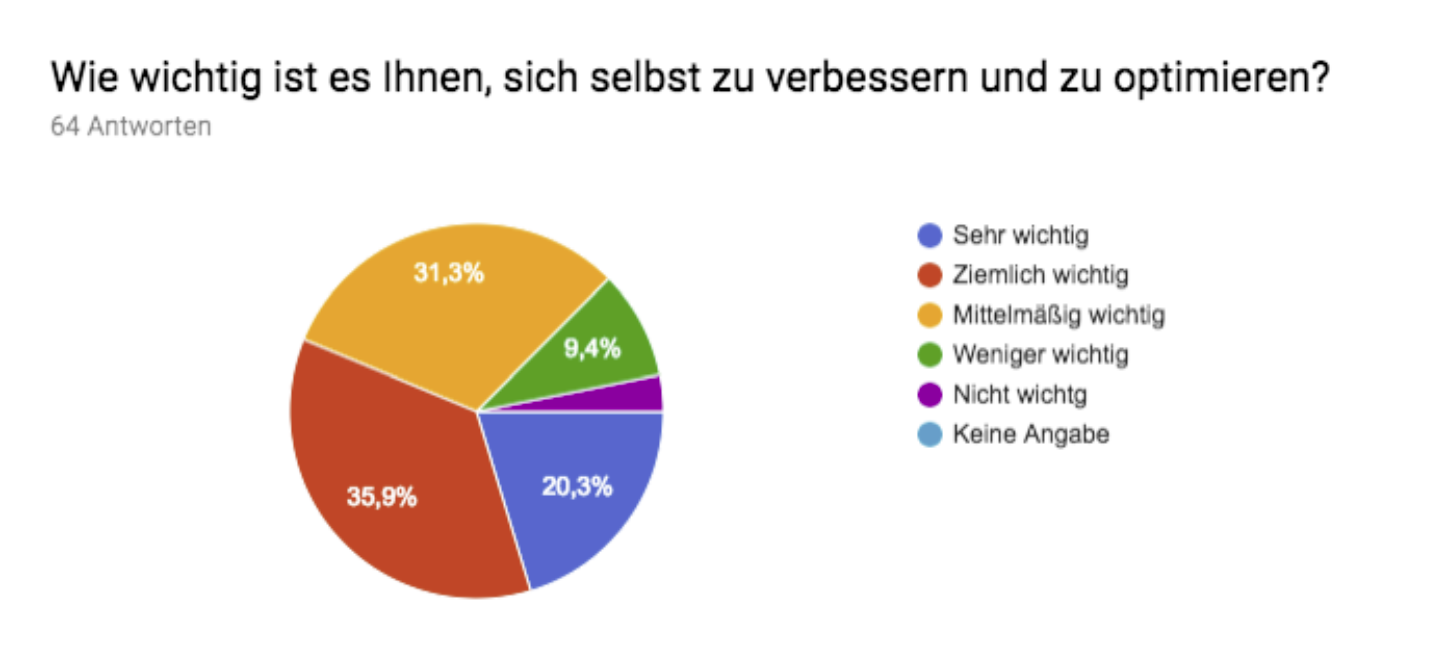
\includegraphics[width=1.0\textwidth]{src/img/kathrin1.png}
  \caption{Diagramm zu den Antworten der Frage: \enquote{Wie wichtig ist es
  Ihnen, sich selbst zu verbessern und zu optimieren?}}
  \label{img:kathrin1}
\end{figure}

Selbstoptimierung ist für 36 von 64 (56,3\%) sehr oder ziemlich wichtig, 20
mittelmäßig wichtig und für 8 (12,5\%) weniger oder nicht wichtig, wobei sich
keine Auffälligkeiten für die verschiedenen Geschlechter, Altersgruppen oder
Technikvorerfahrungen gibt.

Mit 39 Nennungen ist Bildung der stärkste Bereich, in dem die Befragten sich
verbessern, gefolgt von Sport (35) und Ernährung (29). 24 Personen geben an
sich beim Zeit- und Selbstmanagement, 21 Personen beim Sprache(n) lernen und
5 in kleinem Bereich zu optimieren.

Bei der Verwendung technischer Hilfsmittel liegt das Smartphone mit 39
Nennungen vorne, danach folgen Wearables (10) und die Sprachsteuerung (4).
Aus 8 Freitextantworten ergeben sich folgende Hilfsmittel: PC bzw. Computer,
Bücher, Fachliteratur, Meditation, Medikamente, Excel, Websites oder
Empfehlungen. 18 Befragte geben an keine Hilfsmittel zu nutzen.

Die Auswertung zur Häufigkeit der Hilfsmittelnutzung zeigt, dass drei
Antwortmöglichkeiten dominieren: mehrmals am Tag mit 14 (21,9\%), mehrmals in
einer Woche mit 17 (26,6\%) und gar nicht mit 16 (25\%).

\begin{figure}[H]
  \centering
  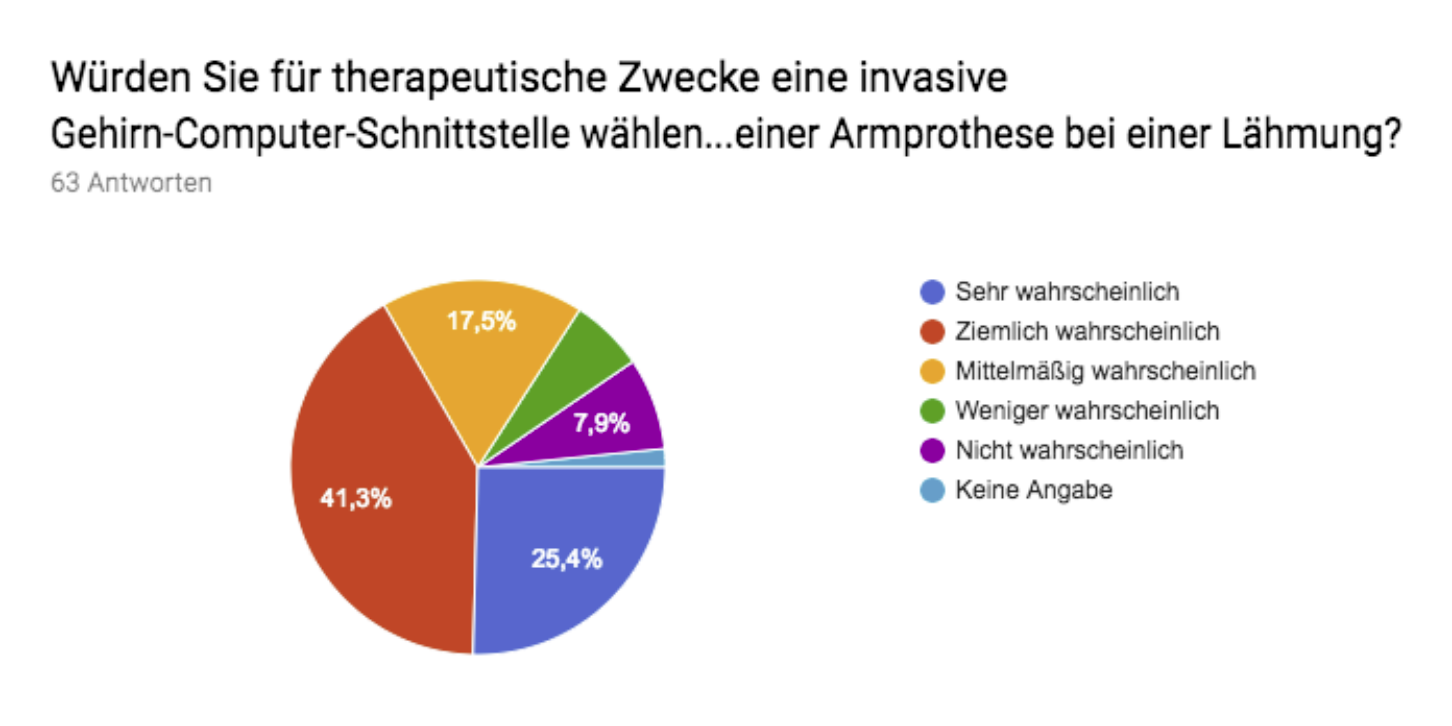
\includegraphics[width=1.0\textwidth]{src/img/kathrin2.png}
  \caption{Diagramm zu den Antworten der Frage: \enquote{Würden Sie für
  therapeutische Zwecke eine invasive Gehirn-Computer-Schnittstelle wählen
  ...?}}
  \label{img:kathrin2}
\end{figure}

Für therapeutische Zwecke würden 42 von 63 (66,7\%) sehr oder ziemlich
wahrscheinlich, eine invasive BCI wählen. Damit ist der Prozentsatz hier
höher als bei der Frage zur Selbstoptimierung, vermutlich durch den
Ausgangspunkt einer Krankheit oder Behinderung. 11 antworten mit mittelmäßig
wahrscheinlich, 9 (14,3\%) mit weniger oder nicht wichtig . Eine leichte
Abweichung gibt es bei den Geschlechtern: bei Männer sind die Angaben sehr
oder ziemlich wahrscheinlich etwas höher, 27 von 38 (71,1\%), als bei den
Frauen, 13 von 20 (65\%). Für die Altersgruppen und Technikvorerfahrungen sind
keine Unterschiede zu erkennen.

\begin{figure}[H]
  \centering
  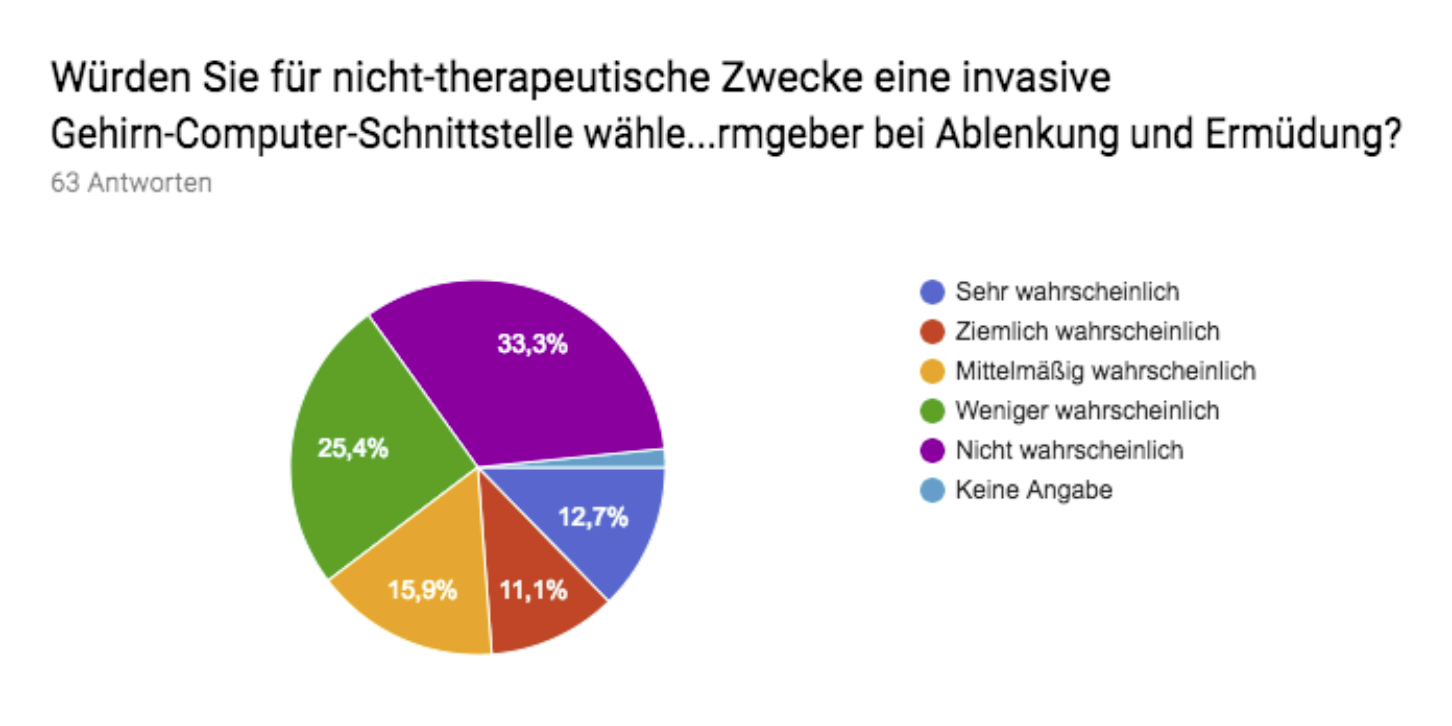
\includegraphics[width=1.0\textwidth]{src/img/kathrin3.png}
  \caption{Diagramm zu den Antworten der Frage: \enquote{Würden Sie für
  nicht-therapeutische Zwecke eine invasive Gehirn-Computer-Schnittstelle
  wählen ...?}}
  \label{img:kathrin3}
\end{figure}

Bei den Antworten zur Verwendung einer invasiven BCI für nicht-therapeutische
Zwecke zeigt sich ein fast umgekehrtes Bild, 15 von 63 (23,8\%) nennen sehr
oder ziemlich wahr- scheinlich, 10 mittelmäßig und 37 (58,7\%) weniger oder
nicht wahrscheinlich. Diese ausgeprägte Zurückhaltung variiert stark
innerhalb der Geschlechter, Altersgruppen und Technikvorerfahrungen. Männer
sind offener für die nicht-therapeutische Verwendung, 12 von 38 (31,6\%)
antworten sehr oder ziemlich wahrscheinlich. Bei Frauen schneit es große
Skepsis beim Einsatz bei einem gesunden Menschen zu geben: 14 von 20 (70\%)
sagen weniger oder nicht wahrscheinlich.

\begin{figure}[H]
  \centering
  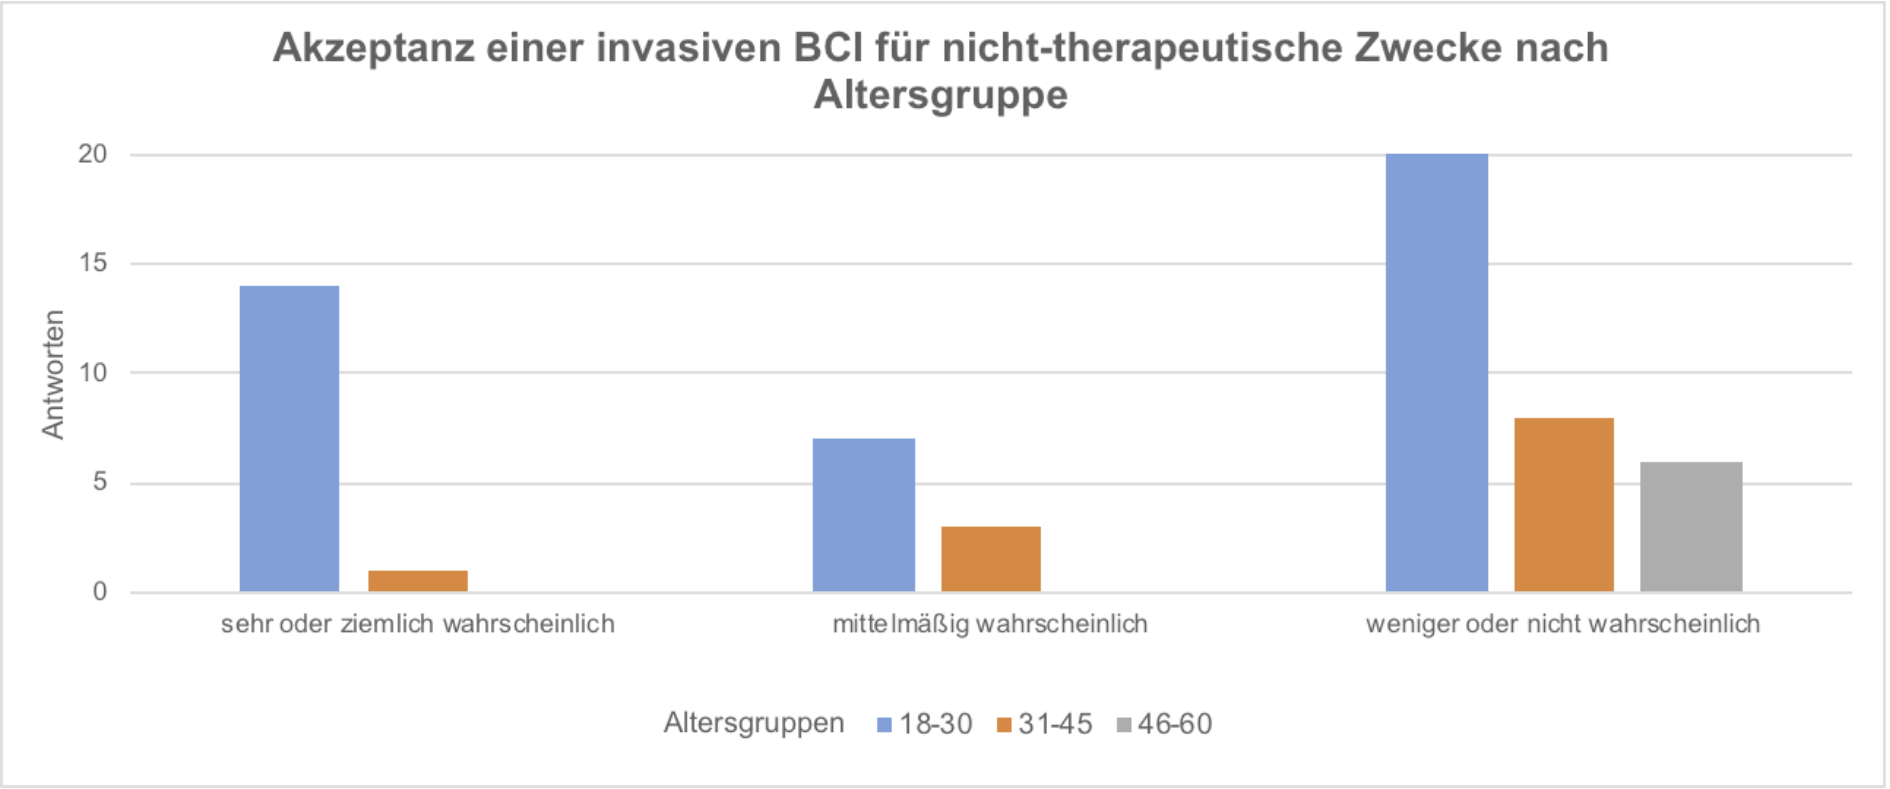
\includegraphics[width=1.0\textwidth]{src/img/kathrin4.png}
  \caption{Akzeptanz einer invasiven BCI für nicht-therapeutische Zwecke nach
  Altersgruppe}
  \label{img:kathrin4}
\end{figure}

Für die Altersgruppen lässt sich sagen, dass mit steigendem Alter die
Akzeptanz deutlich sinkt. In der Altersgruppe 46-60 ist die Basis mit 6
Antworten gering.

\begin{figure}[H]
  \centering
  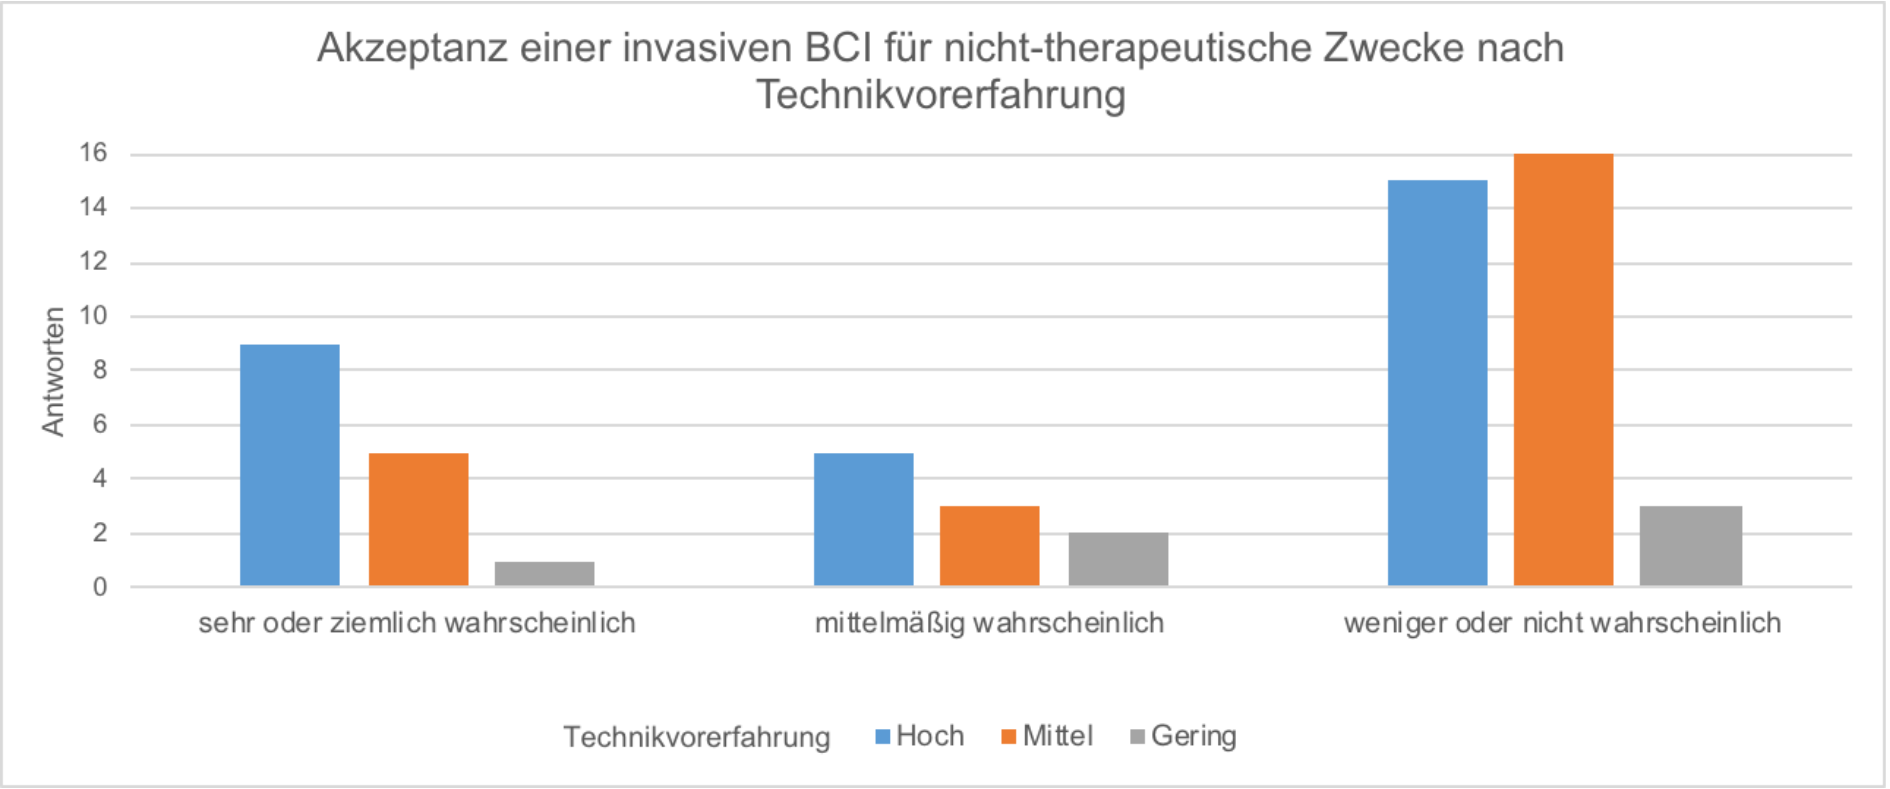
\includegraphics[width=1.0\textwidth]{src/img/kathrin5.png}
  \caption{Akzeptanz einer invasiven BCI für nicht-therapeutische Zwecke nach
  Technikvorerfahrung}
  \label{img:kathrin5}
\end{figure}

Ebenso korreliert die Akzeptanz mit der Technikvorerfahrung. Für die
Technikvorerfahrung \enquote{Gering} ist die Basis mit 6 Antworten klein.
Die etwas komplexere Frage zur Risikobewertung haben 62 Personen beantwortet.
Die Risiken werden absteigend nach den Nennungen für sehr hohes oder hohes
Risiko aufgeführt. Als stärkstes Risiko wird der Missbrauch von im Gehirn
erhobenen Daten angesehen, 43 (69,4\%) geben dafür an. Die Klärung der
Verantwortung bei Schädigung Dritter und das Risiko von Ungerechtigkeit sind
mit 38 bzw. 37 Nennungen (61,3\% bzw. 60,0\%) ähnlich bewertet. Bei den
medizinischen Risiken sind es 32 Antworten (51,6\%), allerdings ist der Wert
für das mittelmäßige Risiko mit 21 hier hoch. Danach folgt das Risiko zur
Ausgrenzung von Individuen und Gruppen, hier sind es 29 (46,8\%). Am wenigsten
bedrohlich werden die unbefugte Steuerung von Außen und die Veränderung der
eigenen Persönlichkeit wahrgenommen, 23 bzw. 21 gaben dies an (37,0\% bzw.
33.9\%). Bei beiden ist sind die Nennung für das mittelmäßige Risiko mit 24
bzw. 22 stark ausgeprägt.

\subsection{Zusammenfassung}
\label{subsec:kathrin_zusammenfassung}
Zu Human Enhancement und der Verwendung von BCIs gibt es eine Vielzahl von
ethischen Aspekten. Deren Reflektion kann helfen, das BCIs eine breite
Akzeptanz in der Gesellschaft finden. Die Analyse der Umfragewerte hat
ergeben, dass der befragte Personenkreis Selbstoptimierung zu 50\% als
ziemlich oder sehr wichtig bewertet und nur für wenige einen kleinen oder gar
keinen Stellenwert hat. Noch höher ist die Akzeptanz von BCIs zu
therapeutischen Zwecken mit 67\%, vermutlich aus der Not einer Krankheit oder
Behinderung heraus. Bei der Verwendung von BCIs bei gesunden Menschen zur
Selbstoptimierung dreht sich das Bild, nur noch 24\% haben eine bejahende
Einstellung zur Verwendung. Bei dieser Frage gibt es große Unterschiede
innerhalb der Geschlechter, Altersgruppen und Technikvorerfahrungen.

\pagebreak
\section{Schlussteil}
Ob Menschen wirklich auf dem Weg zum Cyborg sind, kann hier nicht beantwortet
werden. Jedoch gibt es viele Anzeichen die aufzeigen, dass BCIs eine gängige
Technologie im medizinischen Umfeld werden können. Akzeptanz und
Marktfähigkeit werden vor allem dafür ausschlaggebend sein, ob BCIs auch in
den Alltag Einzug halten.

Es wurden invasive und non-invasive Messverfahren von Gehirnströmen erklärt.
Daraufhin wurden die Vor- und Nachteile der verschiedenen Vorgehensweisen
verglichen. Die invasive Methode wird letzten Endes, trotz hoher
Gesundheitsrisiken vorgezogen, weil die benötigte Präzision nicht durch
andere Verfahren zu erreichen ist.

Moderne Neuroprothesen sind stark von den Erkenntnissen in der Robotik
beeinflusst. Sowohl bei den Steuerungsvorgängen zwischen Mensch und Maschine,
als auch bei der mechatronischen Realisierung von Roboterteilen, die
letztlich als Ersatz für verlorene menschliche Gliedmaßen dienen können. Die
Konstruktion solcher Teile erfordert ein hohes Maß an interdisziplinären
Wissen und bildet komplexe Robotersysteme, mit deren Hilfe sich am Ende
feinmotorische Bewegungen ausführen lassen, die denen des Menschen sehr nahe
kommen. Fragen nach sicherheitstechnischen Anforderungen oder wie die
Steuerung und Prozessführung in Verbindung mit BCIs konkret aussieht blieben
jedoch ungeklärt.

Die Anwendungsmöglichkeiten der BCIs sind dennoch breit gefächert, neben
komplementären Benutzerstatus oder Präzision von Mehrdeutigkeit durchs
Auslesen des Benutzers zu Peripherie, die neben den medizinischen Prothesen
existieren, als auch Neuromarketing welches zeigt, dass wenn es um
Verhaltensforschung geht BCIs hinzugenommen werden können. Wenn es um
außer-medizinische Einsatzgebiete der BCIs geht, ist es schwer deren Nutzen
mit deren heutigen Preisen als nützlich anzusehen. Die Artikel, die sich dazu
geäußert haben, sind einer Meinung, dass die Anwendung im täglichen Leben
erst mit der Bezahlbarkeit der Geräte für den Endverbraucher möglich ist, und
wenn dann nur komplementär mit den bereits etablierten Methoden.

Zu Human Enhancement und der Verwendung von BCIs gibt es eine Vielzahl von
ethischen Aspekten. Deren Reflektion kann helfen, das BCIs eine breite
Akzeptanz in der Gesellschaft finden. Die Analyse der Umfragewerte hat
ergeben, dass der befragte Personenkreis Selbstoptimierung zu 50\% als
ziemlich oder sehr wichtig bewertet und nur für wenige einen kleinen oder gar
keinen Stellenwert hat. Noch höher ist die Akzeptanz von BCIs zu
therapeutischen Zwecken mit 67\%, vermutlich aus der Not einer Krankheit oder
Behinderung heraus. Bei der Verwendung von BCIs bei gesunden Menschen zur
Selbstoptimierung dreht sich das Bild, nur noch 24\% haben eine bejahende
Einstellung zur Verwendung. Bei dieser Frage gibt es große Unterschiede
innerhalb der Geschlechter, Altersgruppen und Technikvorerfahrungen.

Als Fazit ist zu sagen, dass in einem so jungen Themengebiet wie
Gehirn-Computer- Schnittstellen noch vieles offen und vorstellbar ist. Der
medizinische sowie der neurowissenschaftliche Bereich etabliert sich im
Moment und die Anwendungsmöglichkeiten für den Otto-Normal-Verbraucher hinken
noch hinterher.

\pagebreak
\printbibliography[heading=bibintoc]

\pagebreak
\captionsetup[figure]{list=no,labelformat=empty}
\begin{appendices}
  \begin{figure}[H]
    \centering
    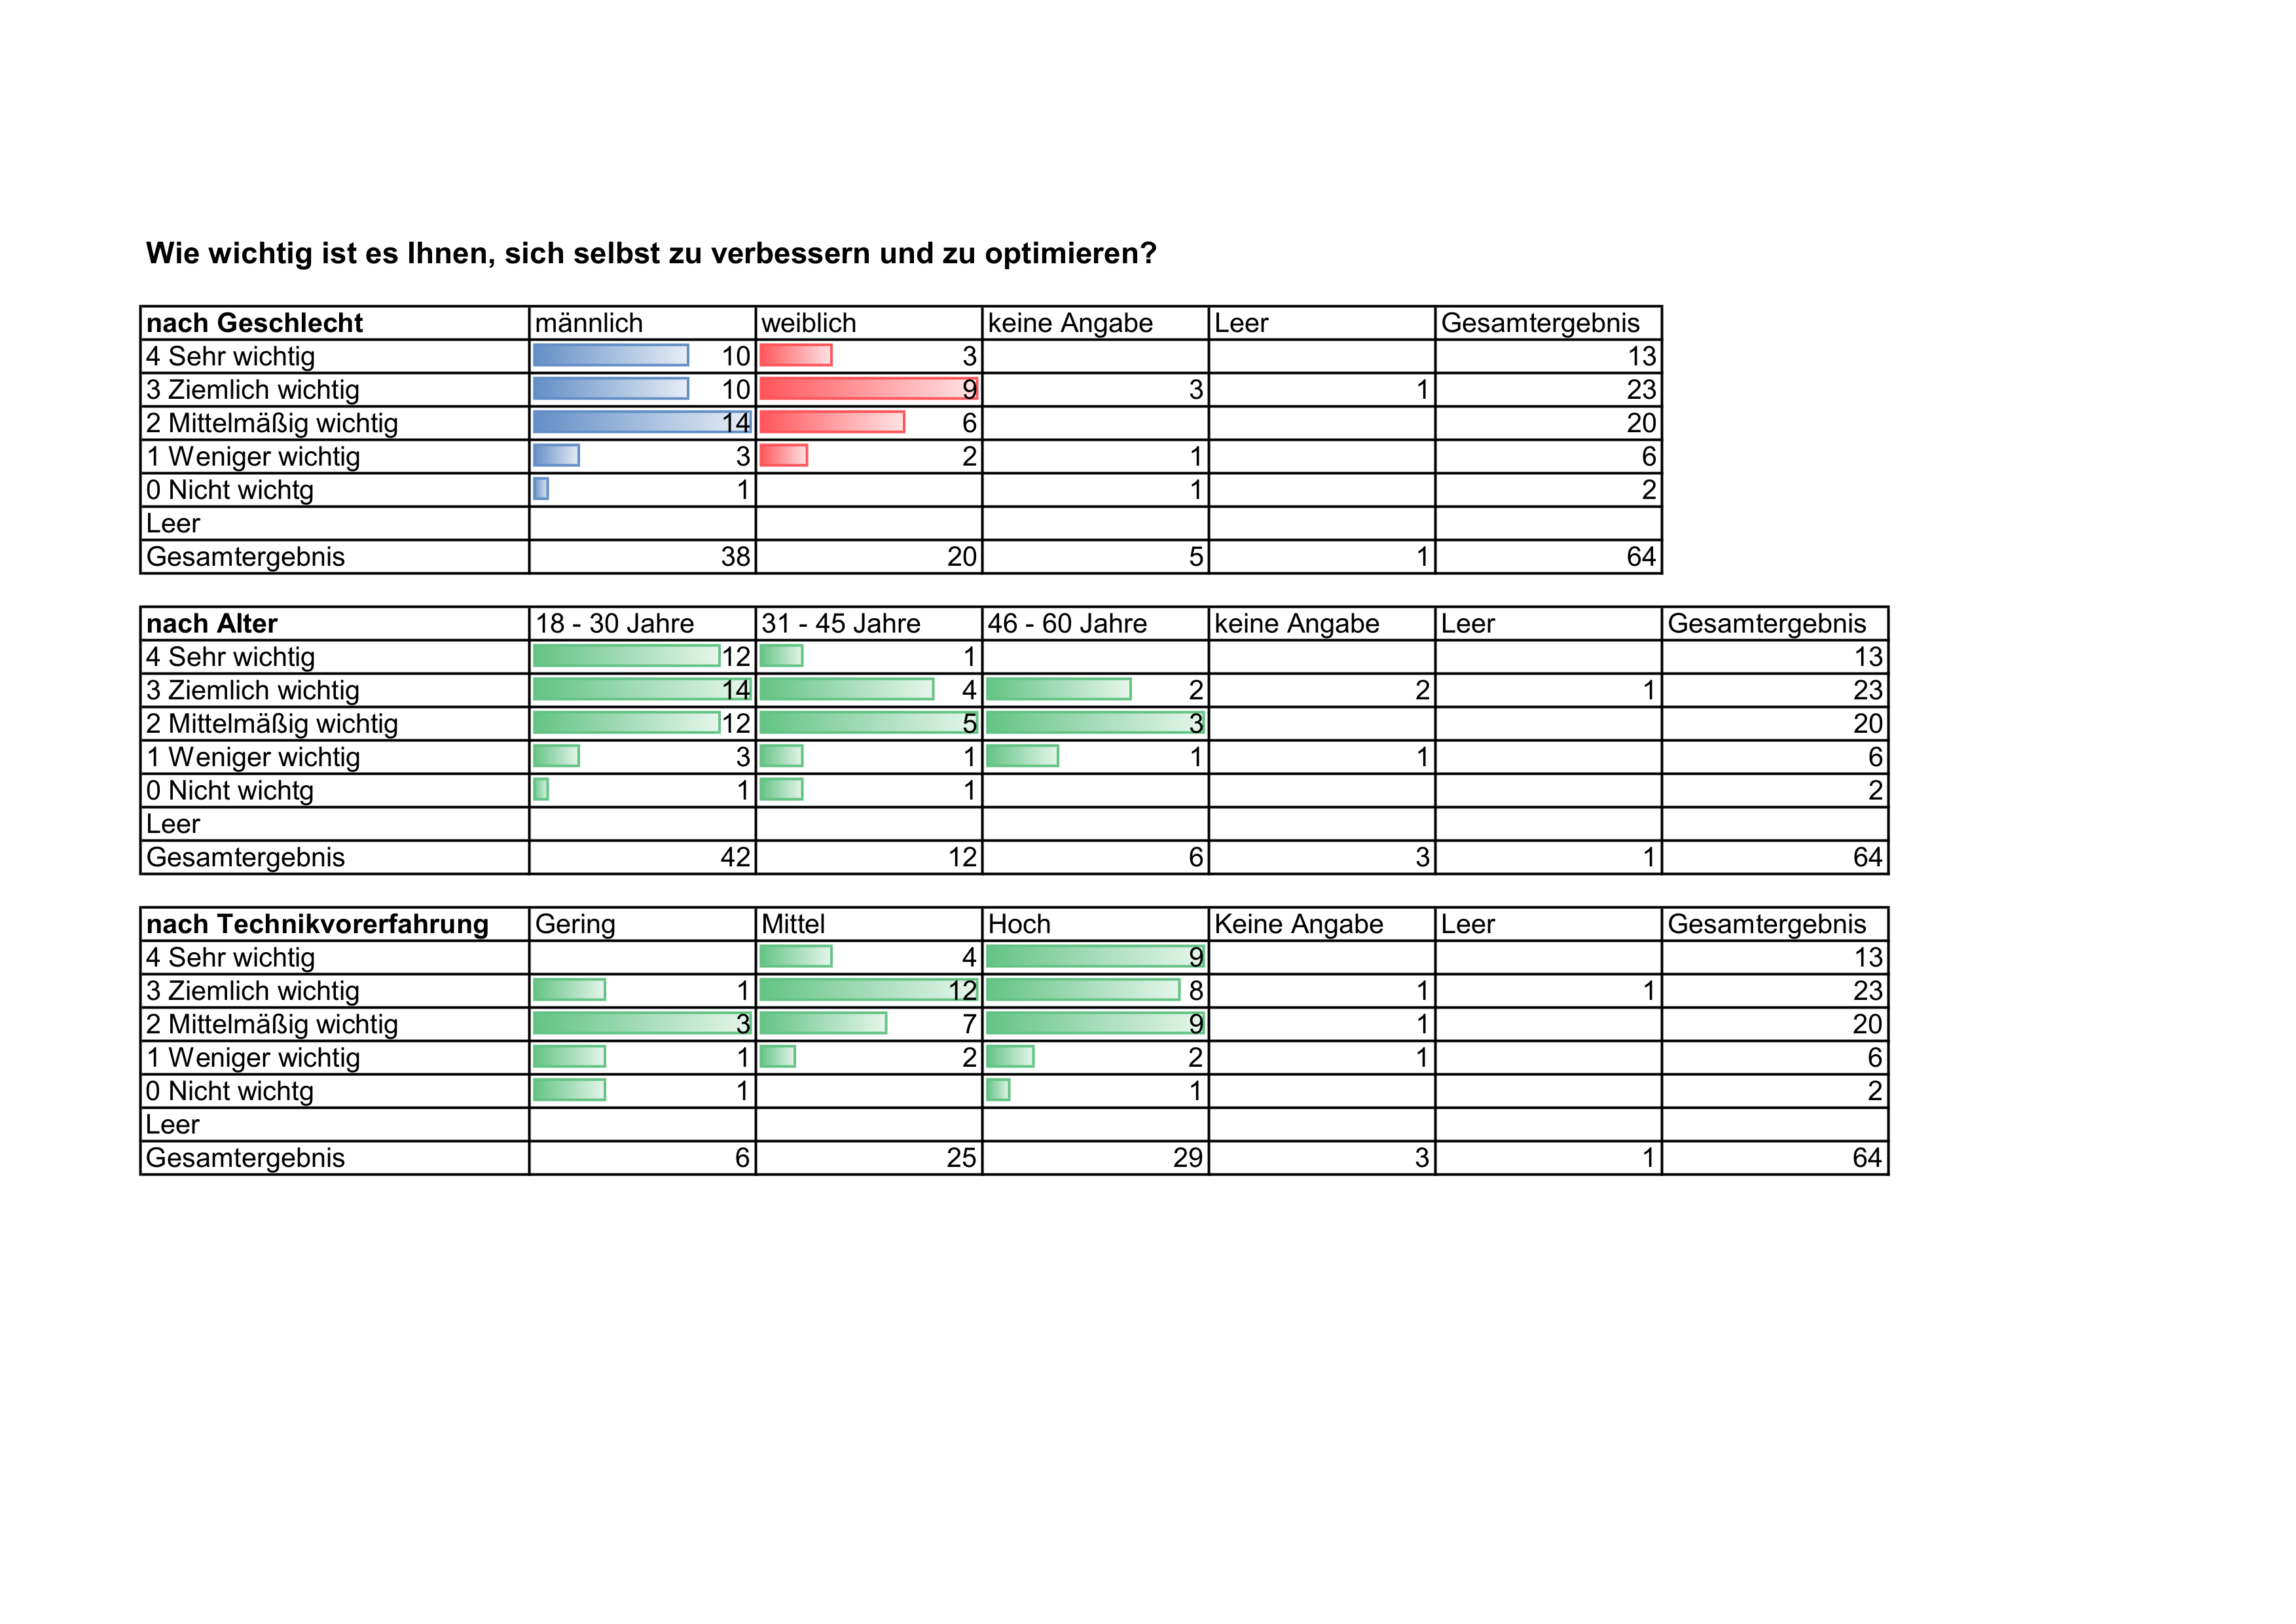
\includegraphics[width=\textwidth,height=\textheight,keepaspectratio]{src/img/kathrin-a1.png}
    \caption{Anlage 1}
  \end{figure}
  \pagebreak

  \begin{figure}[H]
    \centering
    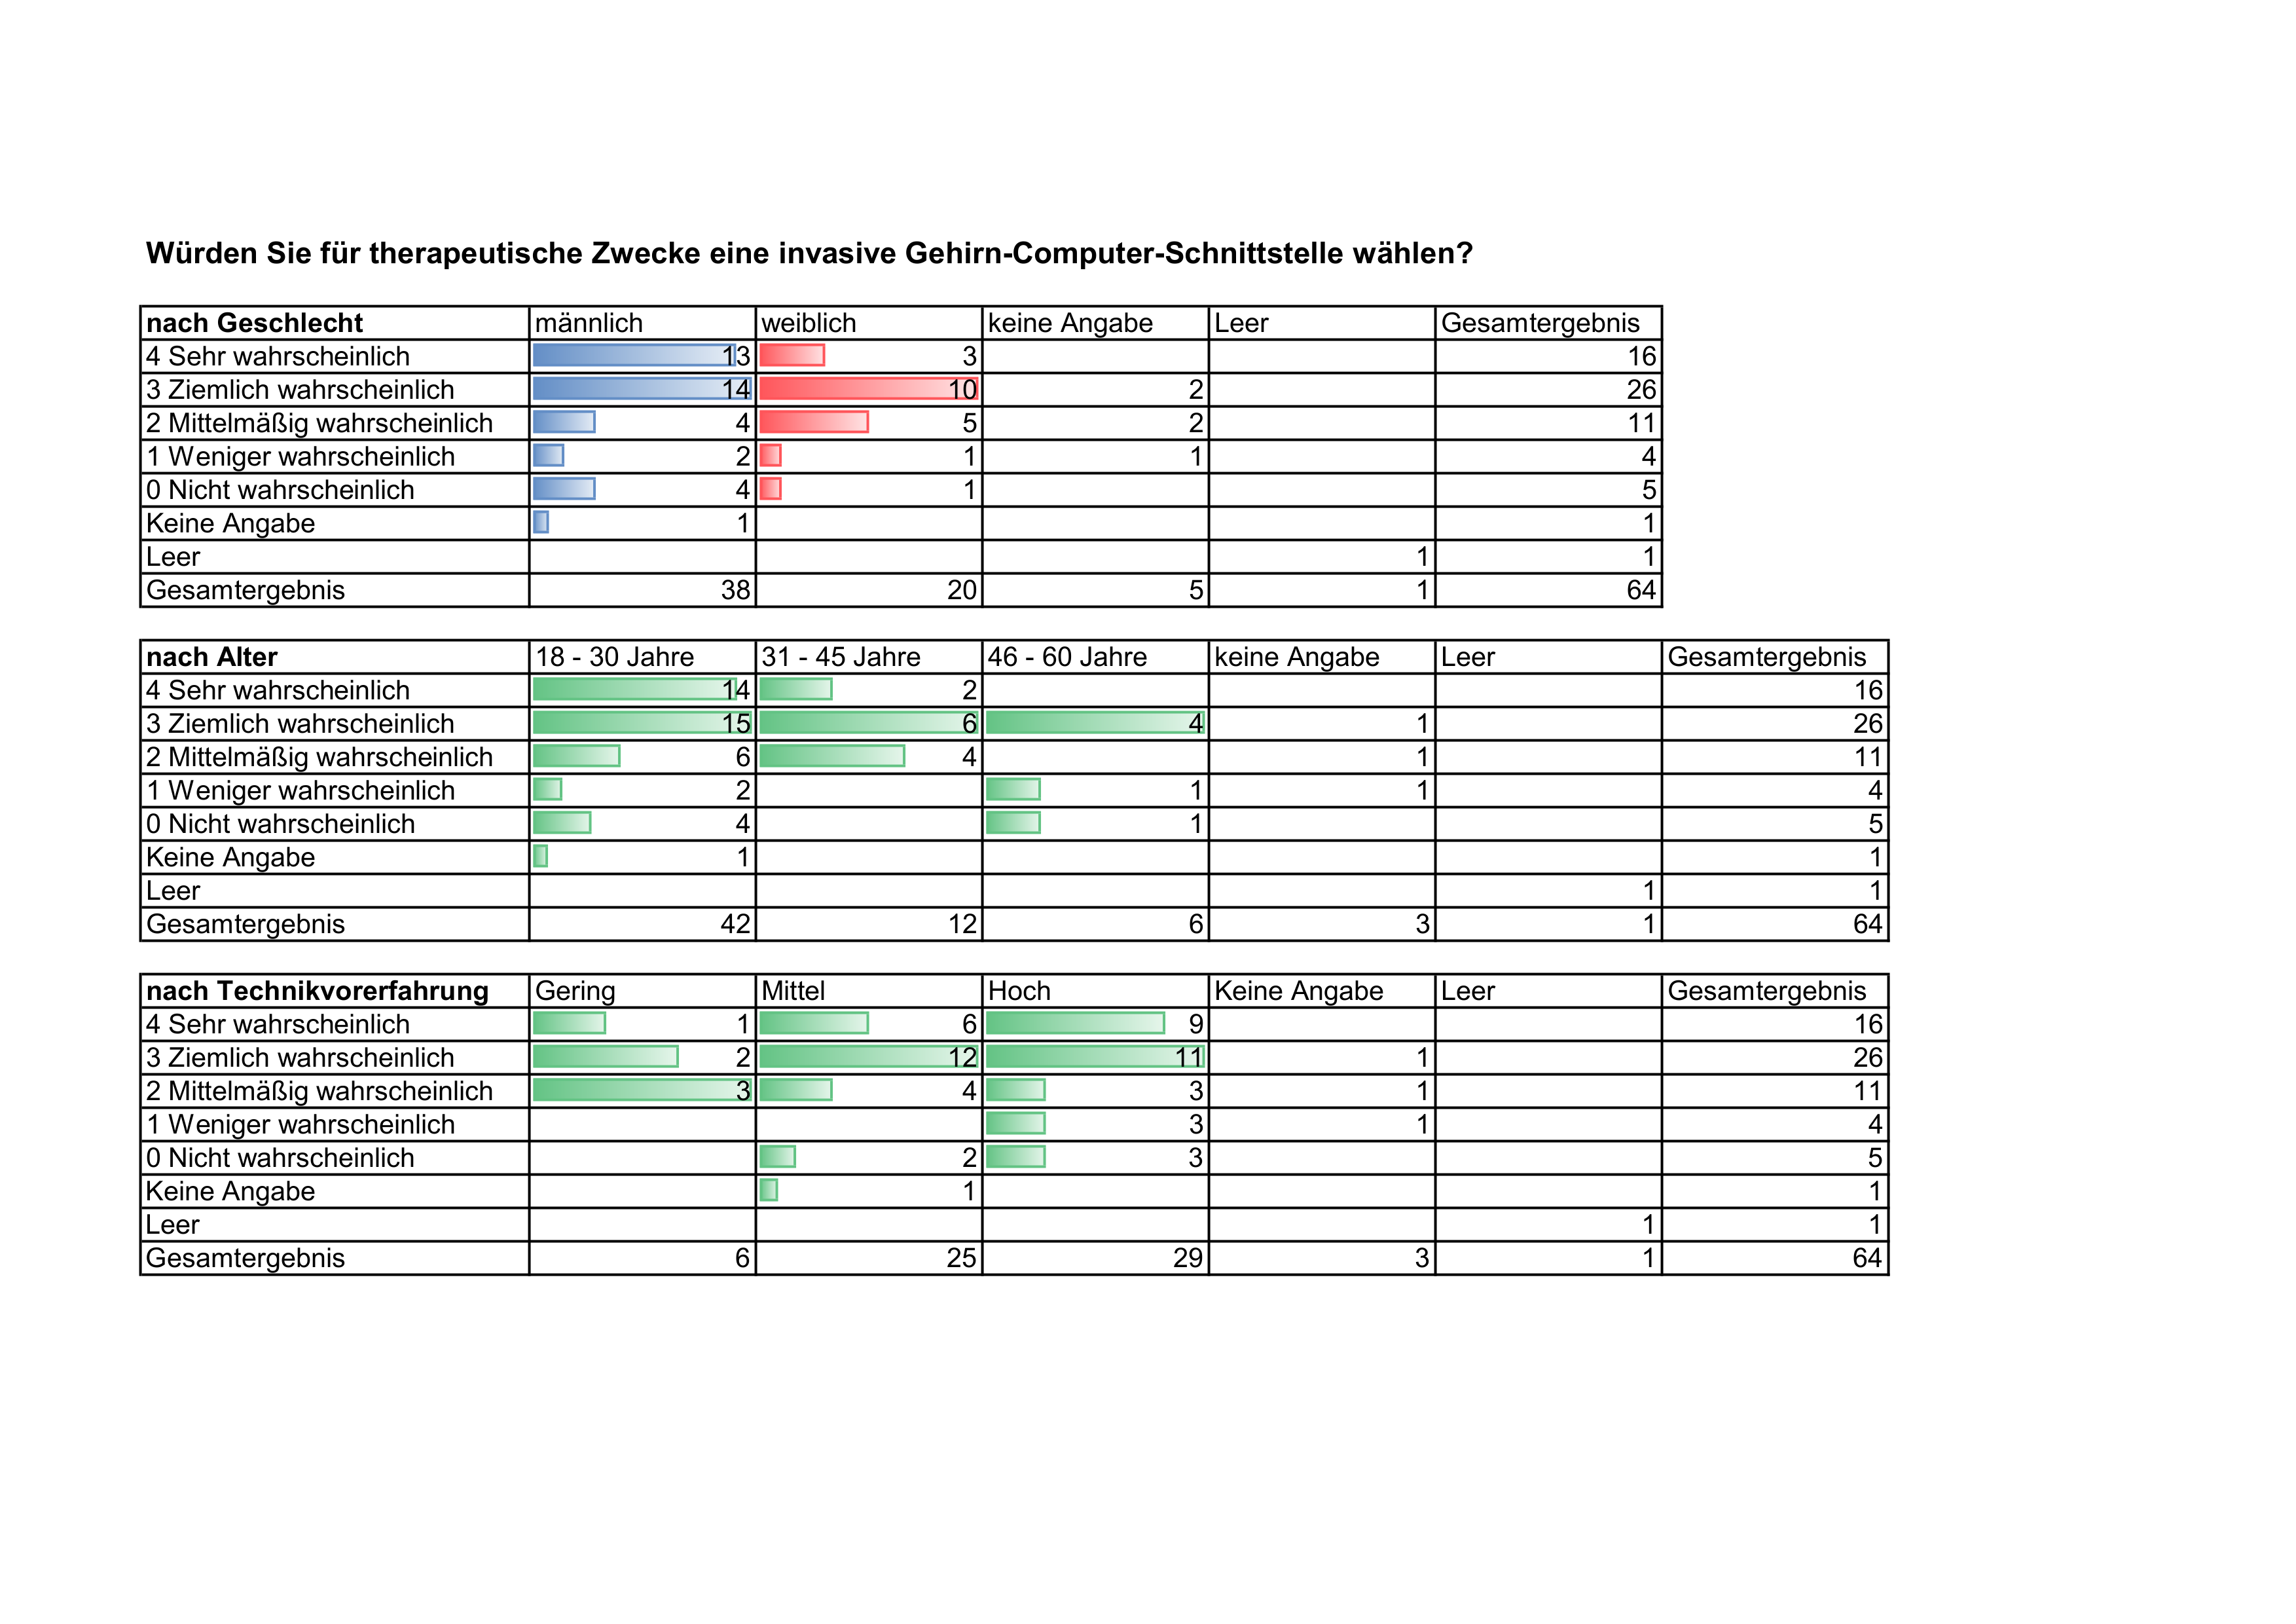
\includegraphics[width=\textwidth,height=\textheight,keepaspectratio]{src/img/kathrin-a2.png}
    \caption{Anlage 2}
  \end{figure}
  \pagebreak

  \begin{figure}[H]
    \centering
    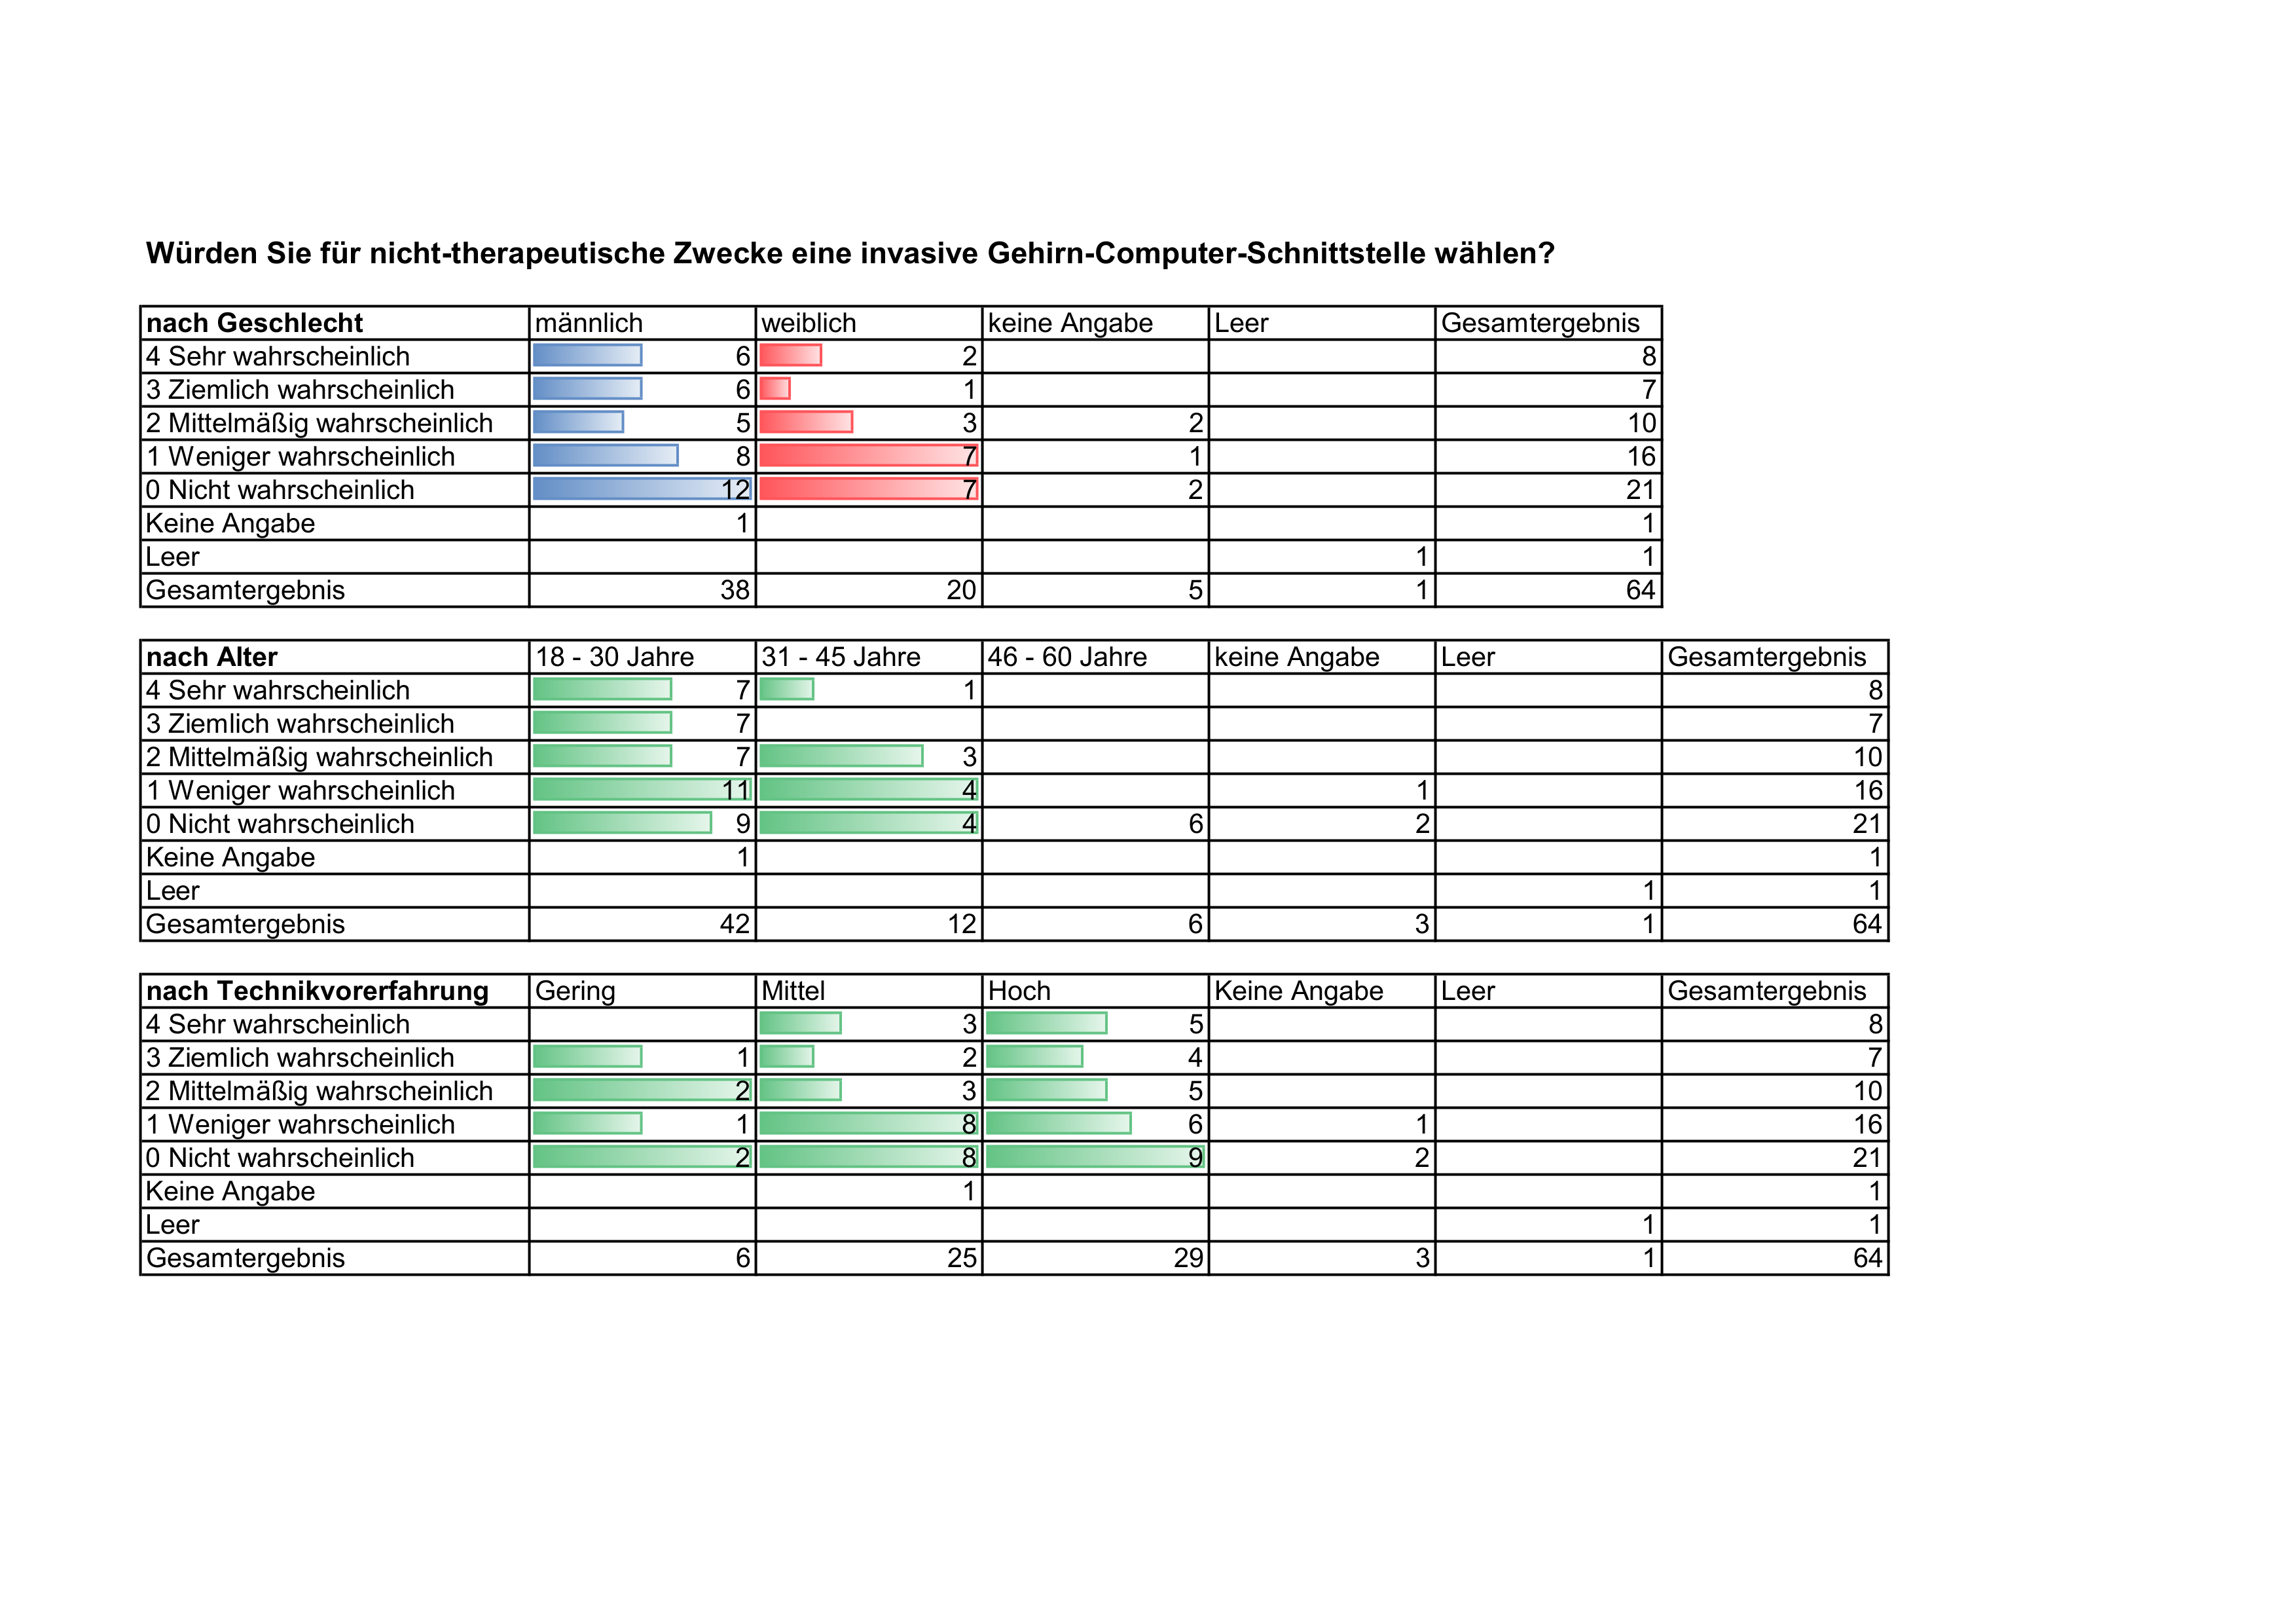
\includegraphics[width=\textwidth,height=\textheight,keepaspectratio]{src/img/kathrin-a3.png}
    \caption{Anlage 3}
  \end{figure}
  \pagebreak

  \begin{figure}[H]
    \centering
    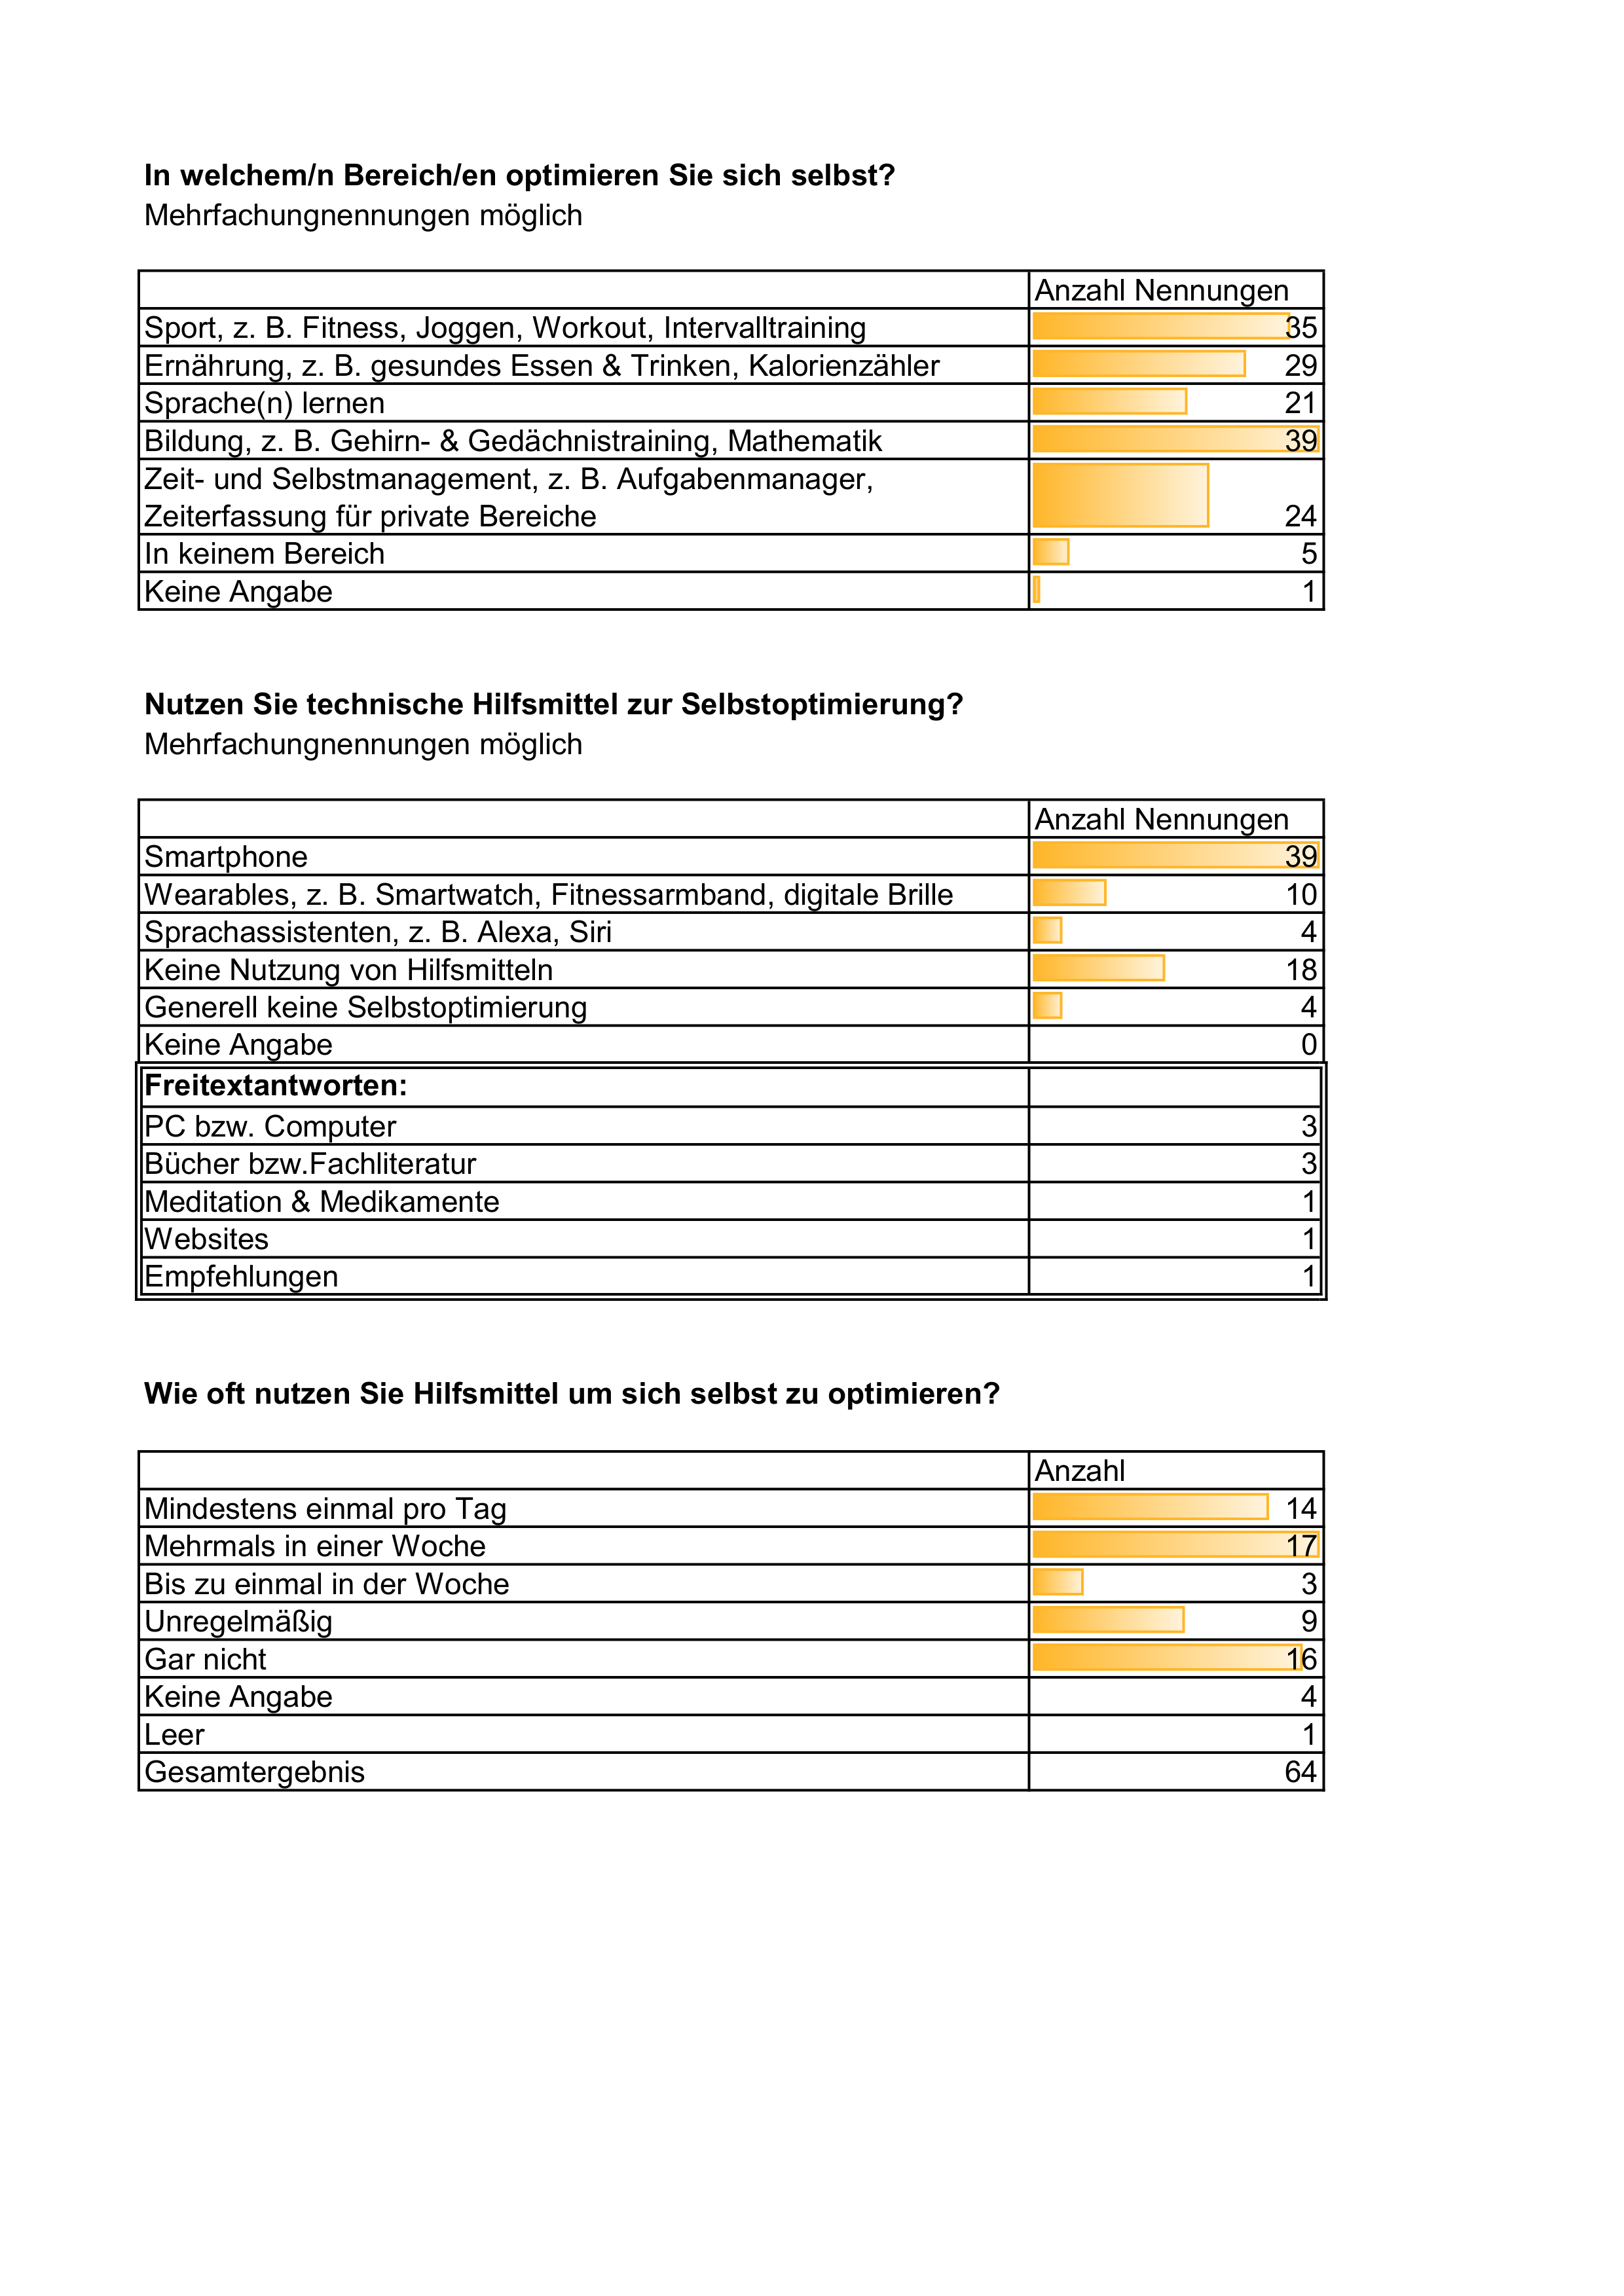
\includegraphics[width=\textwidth,height=\textheight,keepaspectratio]{src/img/kathrin-a4.png}
    \caption{Anlage 4}
  \end{figure}
  \pagebreak

  \begin{figure}[H]
    \centering
    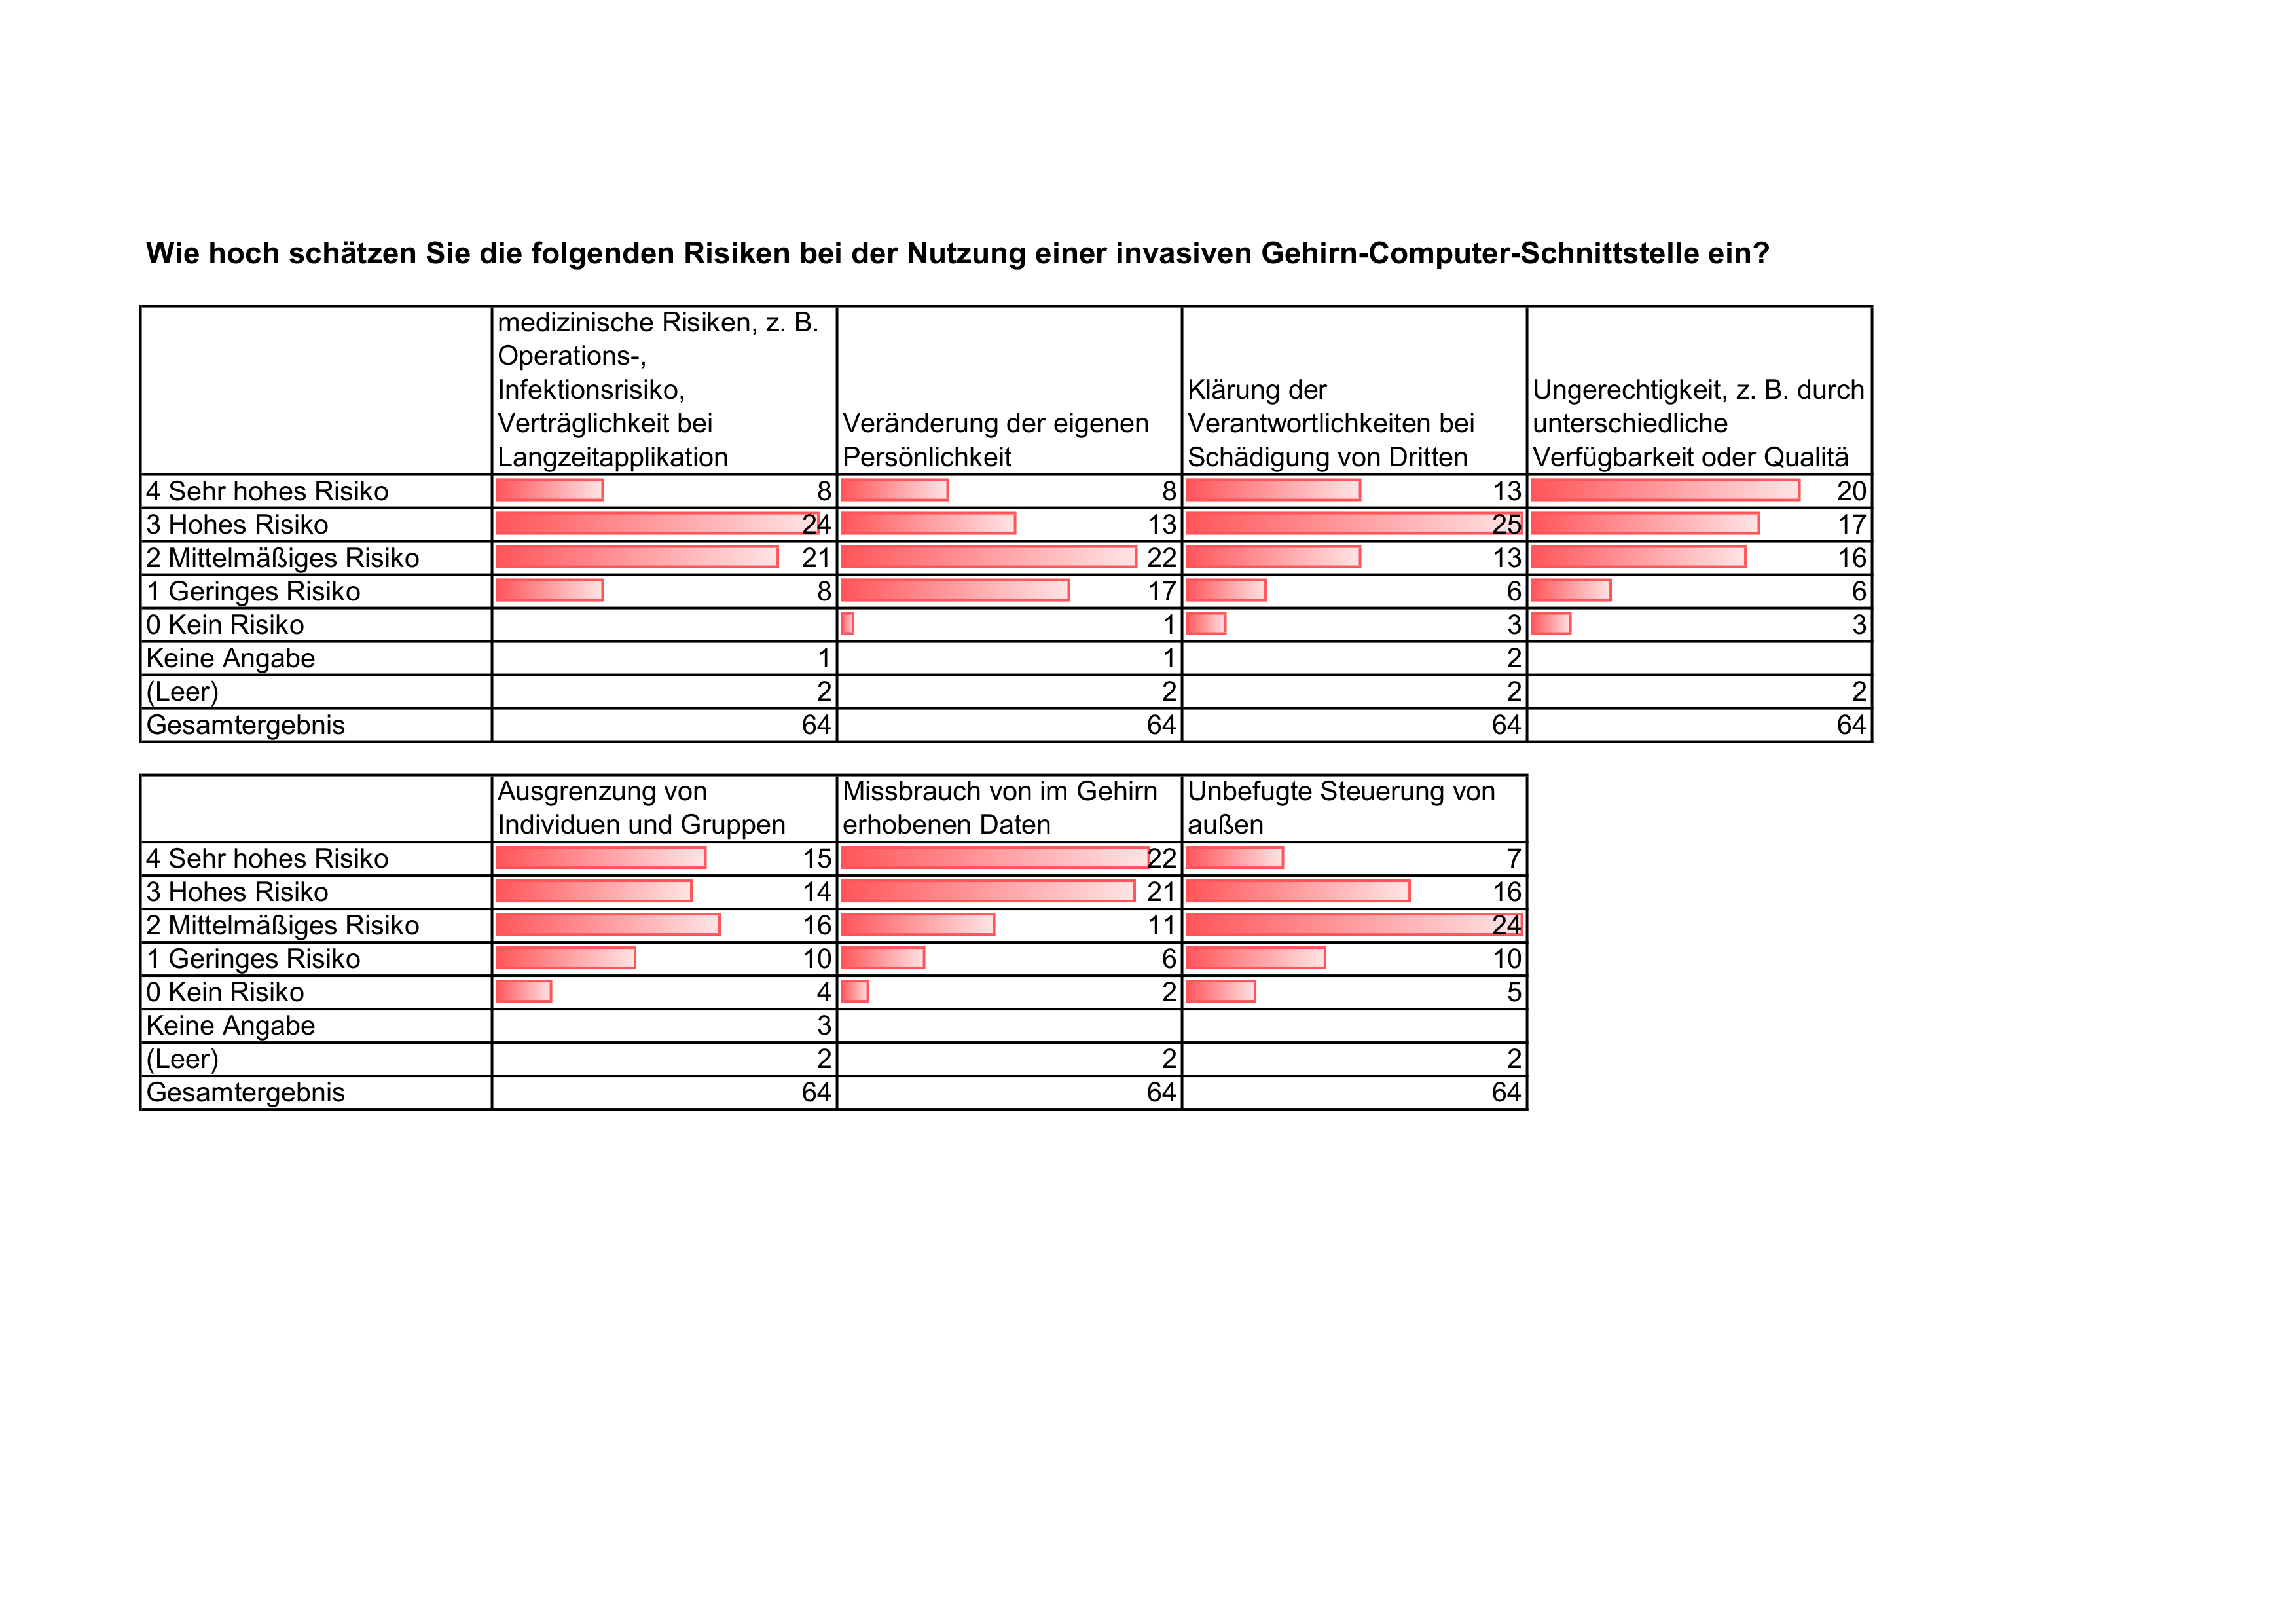
\includegraphics[width=\textwidth,height=\textheight,keepaspectratio]{src/img/kathrin-a5.png}
    \caption{Anlage 5}
  \end{figure}

\end{appendices}

\end{document}
